\section{Implementation and visualization}


\begin{frame}{Node definition}
    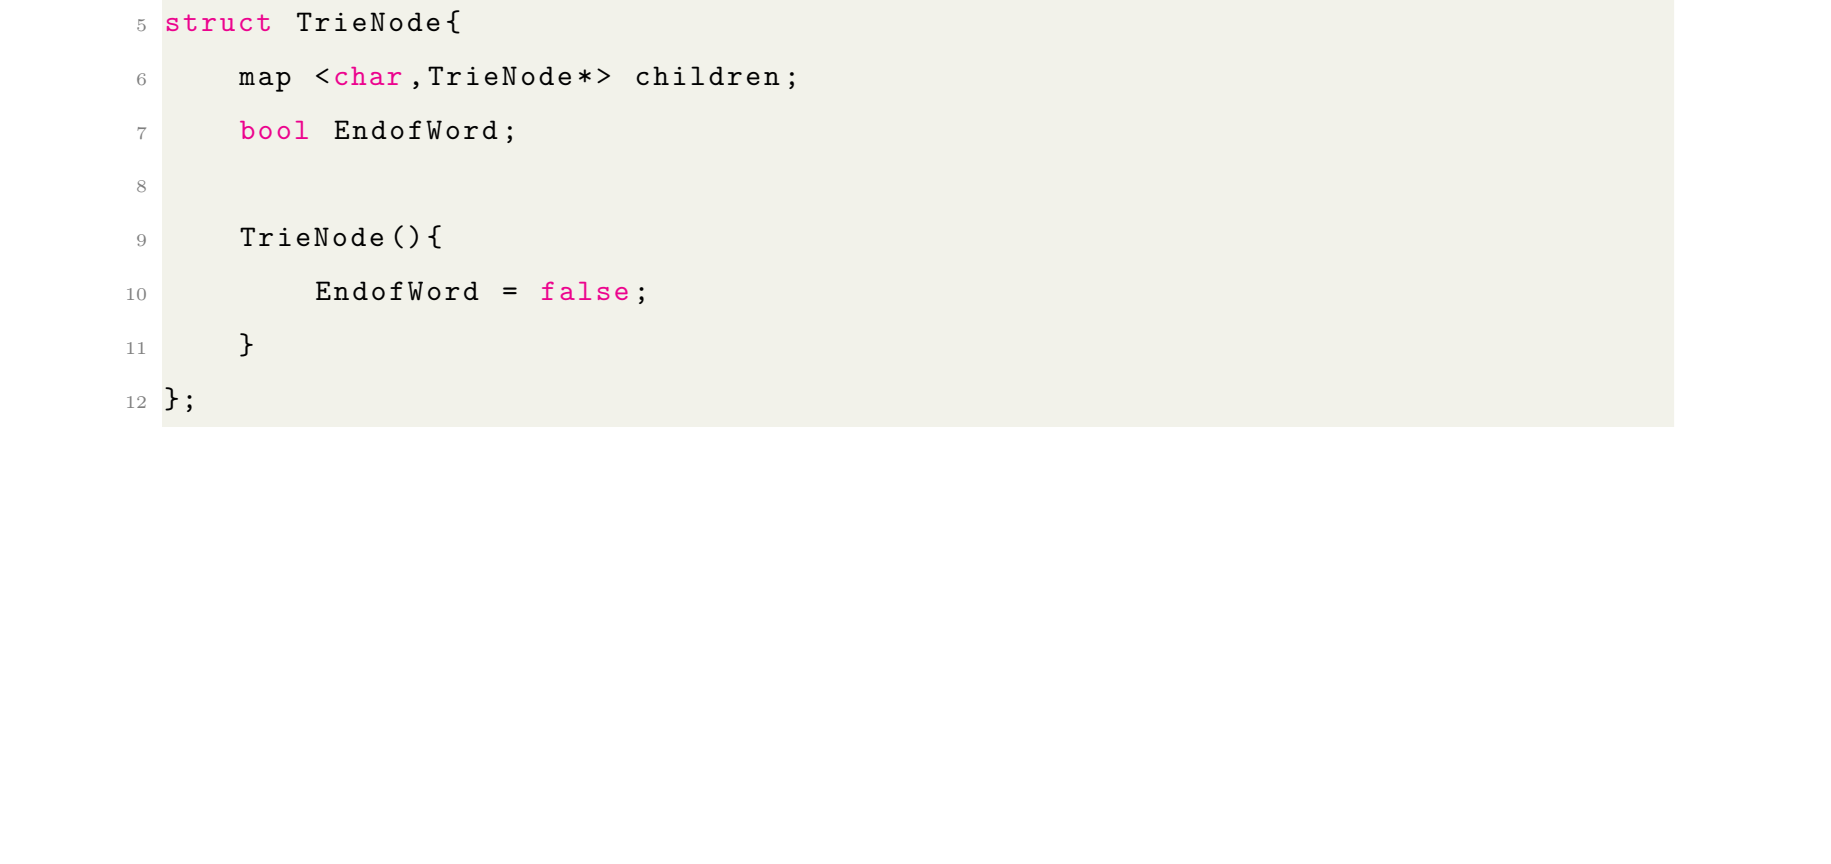
\includegraphics[scale=0.5]{se1.png}

\end{frame}

\begin{frame}{Insert: O(L)}
        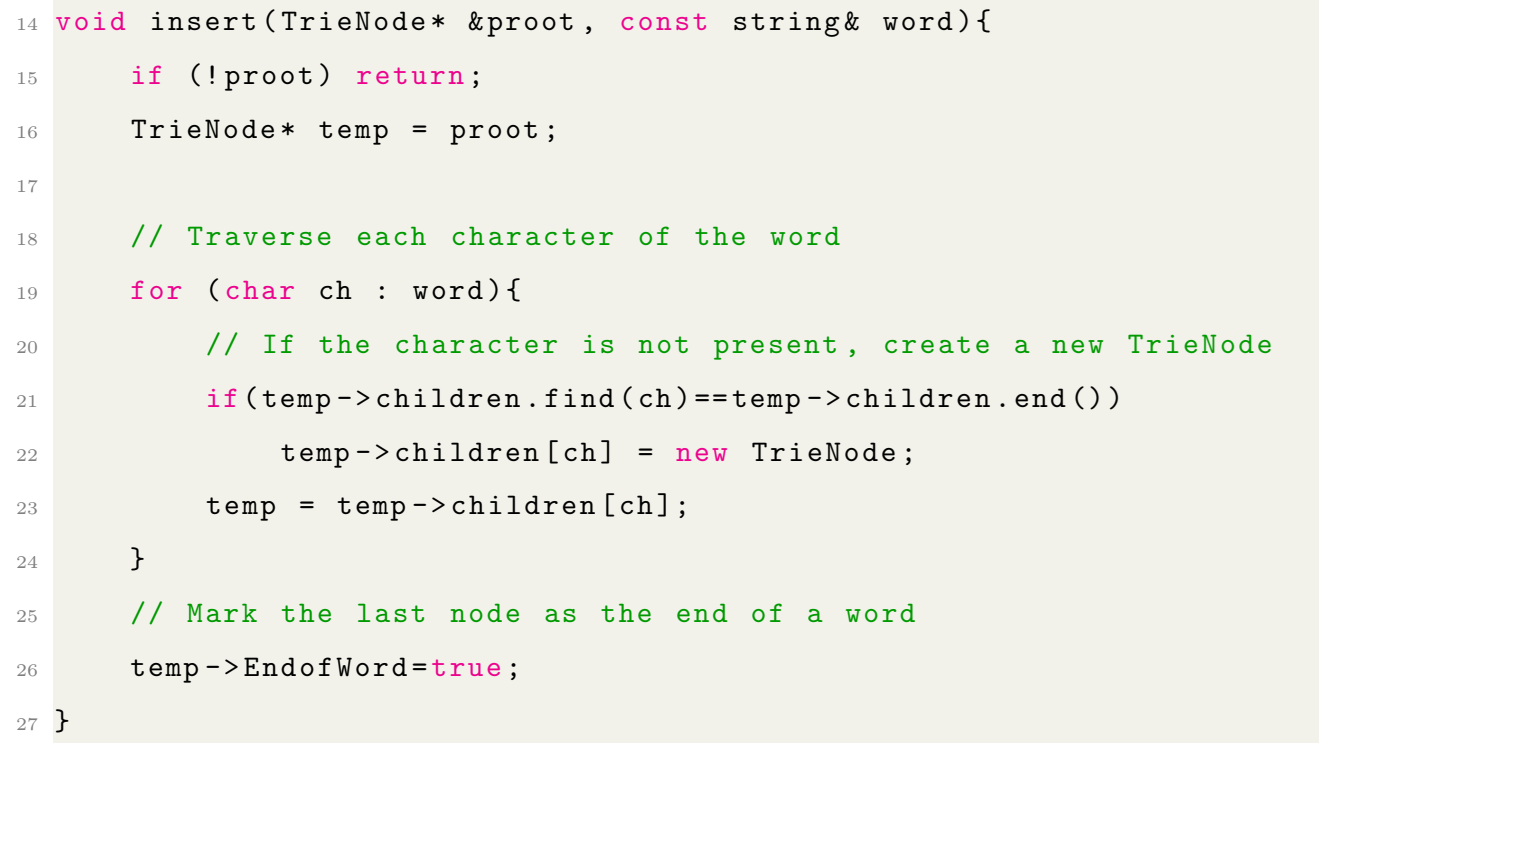
\includegraphics[scale=0.5]{se2.png}

\end{frame}
\begin{frame}{Visualize}
Assume we need to insert 5 words: 
\begin{itemize}[label=$\star$]
    \item app
    \item batman
    \item bat
    \item base
\end{itemize}
\end{frame}

\begin{frame}{Insert "apple"}
\begin{center}
      \begin{tikzpicture}
    \node[ellipse, draw, minimum width=2cm, minimum height=1cm] at (0,0) {Root node};
    \fill[blue] (0,-2) circle (0.5cm);
    \draw (0,-2) circle (0.5cm);
    \node at (0,-2) {\textbf{a}};
    \draw[->] (0,-0.5) -- (0,-1.5);
\end{tikzpicture}
\end{center}
  
\end{frame}
\begin{frame}{Insert "apple"}
    \begin{center}
        \begin{tikzpicture}
   \node[ellipse, draw, minimum width=2cm, minimum height=1cm] at (0,0) {Root node};
   
    \draw (0,-2) circle (0.5cm);
    \node at (0,-2) {\textbf{a}};
    \draw[->] (0,-0.5) -- (0,-1.5);
     \fill[blue] (0,-4) circle (0.5cm);
      \draw (0,-4) circle (0.5cm);
    \node at (0,-4) {\textbf{p}};
    \draw[->] (0,-2.5) -- (0,-3.5);
    
\end{tikzpicture}
    \end{center}
\end{frame}
\begin{frame}{Insert "apple"}
    \begin{center}
        \begin{tikzpicture}
    % Hình elips "Root node"
    \node[ellipse, draw, minimum width=2cm, minimum height=1cm] at (0,0) {Root node};
    
    % Vòng tròn chứa "a" (không tô màu)
    \draw (0,-2) circle (0.5cm);
    \node at (0,-2) {\textbf{a}};
    \draw[->] (0,-0.5) -- (0,-1.5); % Mũi tên từ Root node tới "a"
    
    % Vòng tròn chứa "p" thứ nhất (không tô màu)
    \draw (0,-4) circle (0.5cm);
    \node at (0,-4) {\textbf{p}};
    \draw[->] (0,-2.5) -- (0,-3.5); % Mũi tên từ "a" tới "p"
    
    % Vòng tròn chứa "p" thứ hai (tô màu xanh dương)
    \fill[blue] (0,-6) circle (0.5cm); % Tô màu xanh dương
    \draw (0,-6) circle (0.5cm);
    \node at (0,-6) {\textbf{p}};
    \draw[->] (0,-4.5) -- (0,-5.5); % Mũi tên từ "p" trước tới "p" cuối
\end{tikzpicture}

    \end{center}
\end{frame}
\begin{frame}{Insert "apple"}
    \begin{center}
        \begin{tikzpicture}
    % Hình elips "Root node"
    \node[ellipse, draw, minimum width=2cm, minimum height=1cm] at (0,0) {Root node};
    
    % Vòng tròn chứa "a" (không tô màu)
    \draw (0,-2) circle (0.5cm);
    \node at (0,-2) {\textbf{a}};
    \draw[->] (0,-0.5) -- (0,-1.5); % Mũi tên từ Root node tới "a"
    
    % Vòng tròn chứa "p" thứ nhất (không tô màu)
    \draw (0,-3.5) circle (0.5cm);
    \node at (0,-3.5) {\textbf{p}};
    \draw[->] (0,-2.5) -- (0,-3); % Mũi tên từ "a" tới "p"
    
    % Vòng tròn chứa "p" thứ hai (không tô màu)
    \draw (0,-5) circle (0.5cm);
    \node at (0,-5) {\textbf{p}};
    \draw[->] (0,-4) -- (0,-4.5); % Mũi tên từ "p" trước tới "p"
    
    % Vòng tròn chứa "l" (tô màu xanh dương)
    \fill[blue] (0,-6.5) circle (0.5cm); % Tô màu xanh dương
    \draw (0,-6.5) circle (0.5cm);
    \node at (0,-6.5) {\textbf{l}};
    \draw[->] (0,-5.5) -- (0,-6); % Mũi tên từ "p" tới "l"
\end{tikzpicture}
    \end{center}
\end{frame}
\begin{frame}{Insert "apple"}
\begin{center}
    \begin{tikzpicture}[scale=0.7]
    % Vẽ hình elips chứa "Root node" tại tọa độ (0,0)
    \node[ellipse, draw, minimum width=2cm, minimum height=1cm] at (0,0) {Root node};
    
    % Vẽ vòng tròn chứa "a" tại (0,-2), không tô màu
    \draw (0,-2) circle (0.5cm);
    \node at (0,-2) {\textbf{a}}; % Chữ "a" in đậm ở tâm vòng tròn
    \draw[->] (0,-0.7) -- (0,-1.5); % Mũi tên từ dưới "Root node" tới trên "a"
    
    % Vẽ vòng tròn chứa "p" thứ nhất tại (0,-3.5), không tô màu
    \draw (0,-3.5) circle (0.5cm);
    \node at (0,-3.5) {\textbf{p}}; % Chữ "p" in đậm ở tâm vòng tròn
    \draw[->] (0,-2.5) -- (0,-3); % Mũi tên từ dưới "a" tới trên "p"
    
    % Vẽ vòng tròn chứa "p" thứ hai tại (0,-5), không tô màu
    \draw (0,-5) circle (0.5cm);
    \node at (0,-5) {\textbf{p}}; % Chữ "p" in đậm ở tâm vòng tròn
    \draw[->] (0,-4) -- (0,-4.5); % Mũi tên từ dưới "p" trước tới trên "p"
    
    % Vẽ vòng tròn chứa "l" tại (0,-6.5), không tô màu
    \draw (0,-6.5) circle (0.5cm);
    \node at (0,-6.5) {\textbf{l}}; % Chữ "l" in đậm ở tâm vòng tròn
    \draw[->] (0,-5.5) -- (0,-6); % Mũi tên từ dưới "p" tới trên "l"
    
    % Vẽ vòng tròn chứa "e" tại (0,-8), tô màu xanh dương
    \fill[blue] (0,-8) circle (0.5cm); % Tô nền màu xanh dương
    \draw (0,-8) circle (0.5cm); % Vẽ viền vòng tròn
    \node at (0,-8) {\textbf{e}}; % Chữ "e" in đậm ở tâm vòng tròn
    \draw[->] (0,-7) -- (0,-7.5); % Mũi tên từ dưới "l" tới trên "e"
\end{tikzpicture}
\end{center}
\end{frame}
\begin{frame}{Insert "apple"}
\begin{center}
    \begin{tikzpicture}[scale=0.7]
    % Vẽ hình elips chứa "Root node" tại tọa độ (0,0)
    \node[ellipse, draw, minimum width=2cm, minimum height=1cm] at (0,0) {Root node};
    
    % Vẽ vòng tròn chứa "a" tại (0,-2), không tô màu
    \draw (0,-2) circle (0.5cm);
    \node at (0,-2) {\textbf{a}}; % Chữ "a" in đậm ở tâm vòng tròn
    \draw[->] (0,-0.7) -- (0,-1.5); % Mũi tên từ dưới "Root node" tới trên "a"
    
    % Vẽ vòng tròn chứa "p" thứ nhất tại (0,-3.5), không tô màu
    \draw (0,-3.5) circle (0.5cm);
    \node at (0,-3.5) {\textbf{p}}; % Chữ "p" in đậm ở tâm vòng tròn
    \draw[->] (0,-2.5) -- (0,-3); % Mũi tên từ dưới "a" tới trên "p"
    
    % Vẽ vòng tròn chứa "p" thứ hai tại (0,-5), không tô màu
    \draw (0,-5) circle (0.5cm);
    \node at (0,-5) {\textbf{p}}; % Chữ "p" in đậm ở tâm vòng tròn
    \draw[->] (0,-4) -- (0,-4.5); % Mũi tên từ dưới "p" trước tới trên "p"
    
    % Vẽ vòng tròn chứa "l" tại (0,-6.5), không tô màu
    \draw (0,-6.5) circle (0.5cm);
    \node at (0,-6.5) {\textbf{l}}; % Chữ "l" in đậm ở tâm vòng tròn
    \draw[->] (0,-5.5) -- (0,-6); % Mũi tên từ dưới "p" tới trên "l"
    
    % Vẽ vòng tròn chứa "e" tại (0,-8), tô màu xanh dương
    \fill[green] (0,-8) circle (0.5cm); % Tô nền màu xanh dương
    \draw (0,-8) circle (0.5cm); % Vẽ viền vòng tròn
    \node at (0,-8) {\textbf{e}}; % Chữ "e" in đậm ở tâm vòng tròn
    \draw[->] (0,-7) -- (0,-7.5); % Mũi tên từ dưới "l" tới trên "e"
\end{tikzpicture}
\end{center}
\end{frame}
\begin{frame}{Insert "app"}
\begin{center}
    \begin{tikzpicture}[scale=0.7]
    % Vẽ hình elips chứa "Root node" tại tọa độ (0,0)
    \node[ellipse, draw, minimum width=2cm, minimum height=1cm] at (0,0) {Root node};
    
    % Vẽ vòng tròn chứa "a" tại (0,-2), không tô màu
     \fill[blue] (0,-2) circle (0.5cm);
    \draw (0,-2) circle (0.5cm);
    \node at (0,-2) {\textbf{a}}; % Chữ "a" in đậm ở tâm vòng tròn
    \draw[->] (0,-0.7) -- (0,-1.5); % Mũi tên từ dưới "Root node" tới trên "a"
    
    % Vẽ vòng tròn chứa "p" thứ nhất tại (0,-3.5), không tô màu
    \draw (0,-3.5) circle (0.5cm);
    \node at (0,-3.5) {\textbf{p}}; % Chữ "p" in đậm ở tâm vòng tròn
    \draw[->] (0,-2.5) -- (0,-3); % Mũi tên từ dưới "a" tới trên "p"
    
    % Vẽ vòng tròn chứa "p" thứ hai tại (0,-5), không tô màu
    \draw (0,-5) circle (0.5cm);
    \node at (0,-5) {\textbf{p}}; % Chữ "p" in đậm ở tâm vòng tròn
    \draw[->] (0,-4) -- (0,-4.5); % Mũi tên từ dưới "p" trước tới trên "p"
    
    % Vẽ vòng tròn chứa "l" tại (0,-6.5), không tô màu
    \draw (0,-6.5) circle (0.5cm);
    \node at (0,-6.5) {\textbf{l}}; % Chữ "l" in đậm ở tâm vòng tròn
    \draw[->] (0,-5.5) -- (0,-6); % Mũi tên từ dưới "p" tới trên "l"
    
    % Vẽ vòng tròn chứa "e" tại (0,-8), tô màu xanh dương
    \fill[green] (0,-8) circle (0.5cm); % Tô nền màu xanh dương
    \draw (0,-8) circle (0.5cm); % Vẽ viền vòng tròn
    \node at (0,-8) {\textbf{e}}; % Chữ "e" in đậm ở tâm vòng tròn
    \draw[->] (0,-7) -- (0,-7.5); % Mũi tên từ dưới "l" tới trên "e"
\end{tikzpicture}
\end{center}
\end{frame}
\begin{frame}{Insert "app"}
\begin{center}
    \begin{tikzpicture}[scale=0.7]
    % Vẽ hình elips chứa "Root node" tại tọa độ (0,0)
    \node[ellipse, draw, minimum width=2cm, minimum height=1cm] at (0,0) {Root node};
    
    % Vẽ vòng tròn chứa "a" tại (0,-2), không tô màu
     \fill[blue] (0,-3.5) circle (0.5cm);
    \draw (0,-2) circle (0.5cm);
    \node at (0,-2) {\textbf{a}}; % Chữ "a" in đậm ở tâm vòng tròn
    \draw[->] (0,-0.7) -- (0,-1.5); % Mũi tên từ dưới "Root node" tới trên "a"
    
    % Vẽ vòng tròn chứa "p" thứ nhất tại (0,-3.5), không tô màu
    \draw (0,-3.5) circle (0.5cm);
    \node at (0,-3.5) {\textbf{p}}; % Chữ "p" in đậm ở tâm vòng tròn
    \draw[->] (0,-2.5) -- (0,-3); % Mũi tên từ dưới "a" tới trên "p"
    
    % Vẽ vòng tròn chứa "p" thứ hai tại (0,-5), không tô màu
    \draw (0,-5) circle (0.5cm);
    \node at (0,-5) {\textbf{p}}; % Chữ "p" in đậm ở tâm vòng tròn
    \draw[->] (0,-4) -- (0,-4.5); % Mũi tên từ dưới "p" trước tới trên "p"
    
    % Vẽ vòng tròn chứa "l" tại (0,-6.5), không tô màu
    \draw (0,-6.5) circle (0.5cm);
    \node at (0,-6.5) {\textbf{l}}; % Chữ "l" in đậm ở tâm vòng tròn
    \draw[->] (0,-5.5) -- (0,-6); % Mũi tên từ dưới "p" tới trên "l"
    
    % Vẽ vòng tròn chứa "e" tại (0,-8), tô màu xanh dương
    \fill[green] (0,-8) circle (0.5cm); % Tô nền màu xanh dương
    \draw (0,-8) circle (0.5cm); % Vẽ viền vòng tròn
    \node at (0,-8) {\textbf{e}}; % Chữ "e" in đậm ở tâm vòng tròn
    \draw[->] (0,-7) -- (0,-7.5); % Mũi tên từ dưới "l" tới trên "e"
\end{tikzpicture}

\end{center}
\end{frame}
\begin{frame}{Insert "app"}
\begin{center}
    \begin{tikzpicture}[scale=0.7]
    % Vẽ hình elips chứa "Root node" tại tọa độ (0,0)
    \node[ellipse, draw, minimum width=2cm, minimum height=1cm] at (0,0) {Root node};
    
    % Vẽ vòng tròn chứa "a" tại (0,-2), không tô màu
     \fill[blue] (0,-5) circle (0.5cm);
    \draw (0,-2) circle (0.5cm);
    \node at (0,-2) {\textbf{a}}; % Chữ "a" in đậm ở tâm vòng tròn
    \draw[->] (0,-0.7) -- (0,-1.5); % Mũi tên từ dưới "Root node" tới trên "a"
    
    % Vẽ vòng tròn chứa "p" thứ nhất tại (0,-3.5), không tô màu
    \draw (0,-3.5) circle (0.5cm);
    \node at (0,-3.5) {\textbf{p}}; % Chữ "p" in đậm ở tâm vòng tròn
    \draw[->] (0,-2.5) -- (0,-3); % Mũi tên từ dưới "a" tới trên "p"
    
    % Vẽ vòng tròn chứa "p" thứ hai tại (0,-5), không tô màu
    \draw (0,-5) circle (0.5cm);
    \node at (0,-5) {\textbf{p}}; % Chữ "p" in đậm ở tâm vòng tròn
    \draw[->] (0,-4) -- (0,-4.5); % Mũi tên từ dưới "p" trước tới trên "p"
    
    % Vẽ vòng tròn chứa "l" tại (0,-6.5), không tô màu
    \draw (0,-6.5) circle (0.5cm);
    \node at (0,-6.5) {\textbf{l}}; % Chữ "l" in đậm ở tâm vòng tròn
    \draw[->] (0,-5.5) -- (0,-6); % Mũi tên từ dưới "p" tới trên "l"
    
    % Vẽ vòng tròn chứa "e" tại (0,-8), tô màu xanh dương
    \fill[green] (0,-8) circle (0.5cm); % Tô nền màu xanh dương
    \draw (0,-8) circle (0.5cm); % Vẽ viền vòng tròn
    \node at (0,-8) {\textbf{e}}; % Chữ "e" in đậm ở tâm vòng tròn
    \draw[->] (0,-7) -- (0,-7.5); % Mũi tên từ dưới "l" tới trên "e"
\end{tikzpicture}

\end{center}
\end{frame}
\begin{frame}{Insert "app"}
\begin{center}
    \begin{tikzpicture}[scale=0.7]
    % Vẽ hình elips chứa "Root node" tại tọa độ (0,0)
    \node[ellipse, draw, minimum width=2cm, minimum height=1cm] at (0,0) {Root node};
    
    % Vẽ vòng tròn chứa "a" tại (0,-2), không tô màu
     \fill[green] (0,-5) circle (0.5cm);
    \draw (0,-2) circle (0.5cm);
    \node at (0,-2) {\textbf{a}}; % Chữ "a" in đậm ở tâm vòng tròn
    \draw[->] (0,-0.7) -- (0,-1.5); % Mũi tên từ dưới "Root node" tới trên "a"
    
    % Vẽ vòng tròn chứa "p" thứ nhất tại (0,-3.5), không tô màu
    \draw (0,-3.5) circle (0.5cm);
    \node at (0,-3.5) {\textbf{p}}; % Chữ "p" in đậm ở tâm vòng tròn
    \draw[->] (0,-2.5) -- (0,-3); % Mũi tên từ dưới "a" tới trên "p"
    
    % Vẽ vòng tròn chứa "p" thứ hai tại (0,-5), không tô màu
    \draw (0,-5) circle (0.5cm);
    \node at (0,-5) {\textbf{p}}; % Chữ "p" in đậm ở tâm vòng tròn
    \draw[->] (0,-4) -- (0,-4.5); % Mũi tên từ dưới "p" trước tới trên "p"
    
    % Vẽ vòng tròn chứa "l" tại (0,-6.5), không tô màu
    \draw (0,-6.5) circle (0.5cm);
    \node at (0,-6.5) {\textbf{l}}; % Chữ "l" in đậm ở tâm vòng tròn
    \draw[->] (0,-5.5) -- (0,-6); % Mũi tên từ dưới "p" tới trên "l"
    
    % Vẽ vòng tròn chứa "e" tại (0,-8), tô màu xanh dương
    \fill[green] (0,-8) circle (0.5cm); % Tô nền màu xanh dương
    \draw (0,-8) circle (0.5cm); % Vẽ viền vòng tròn
    \node at (0,-8) {\textbf{e}}; % Chữ "e" in đậm ở tâm vòng tròn
    \draw[->] (0,-7) -- (0,-7.5); % Mũi tên từ dưới "l" tới trên "e"
\end{tikzpicture}
\end{center}
\end{frame}
\begin{frame}{Insert "bat"}
\begin{center}
    \begin{tikzpicture}[scale=0.7]
    % Vẽ hình elips chứa "Root node" tại tọa độ (0,0)
    \node[ellipse, draw, minimum width=2cm, minimum height=1cm] at (1,0) {Root node};
    
    % Vẽ vòng tròn chứa "a" tại (0,-2), không tô màu
     \fill[green] (0,-5) circle (0.5cm);
    \draw (0,-2) circle (0.5cm);
    \node at (0,-2) {\textbf{a}}; % Chữ "a" in đậm ở tâm vòng tròn
    \draw[->] (1,-0.7) -- (0,-1.5); % Mũi tên từ dưới "Root node" tới trên "a"
    
    % Vẽ vòng tròn chứa "p" thứ nhất tại (0,-3.5), không tô màu
    \draw (0,-3.5) circle (0.5cm);
    \node at (0,-3.5) {\textbf{p}}; % Chữ "p" in đậm ở tâm vòng tròn
    \draw[->] (0,-2.5) -- (0,-3); % Mũi tên từ dưới "a" tới trên "p"
    
    % Vẽ vòng tròn chứa "p" thứ hai tại (0,-5), không tô màu
    \draw (0,-5) circle (0.5cm);
    \node at (0,-5) {\textbf{p}}; % Chữ "p" in đậm ở tâm vòng tròn
    \draw[->] (0,-4) -- (0,-4.5); % Mũi tên từ dưới "p" trước tới trên "p"
    
    % Vẽ vòng tròn chứa "l" tại (0,-6.5), không tô màu
    \draw (0,-6.5) circle (0.5cm);
    \node at (0,-6.5) {\textbf{l}}; % Chữ "l" in đậm ở tâm vòng tròn
    \draw[->] (0,-5.5) -- (0,-6); % Mũi tên từ dưới "p" tới trên "l"
    
    % Vẽ vòng tròn chứa "e" tại (0,-8), tô màu xanh dương
    \fill[green] (0,-8) circle (0.5cm); % Tô nền màu xanh dương
    \draw (0,-8) circle (0.5cm); % Vẽ viền vòng tròn
    \node at (0,-8) {\textbf{e}}; % Chữ "e" in đậm ở tâm vòng tròn
    \draw[->] (0,-7) -- (0,-7.5); % Mũi tên từ dưới "l" tới trên "e"

    %b
    \fill[blue] (2,-2) circle (0.5cm);
    \draw (2,-2) circle (0.5cm);
    \node at (2,-2) {\textbf{b}}; % Chữ "a" in đậm ở tâm vòng tròn
    \draw[->] (1,-0.7) -- (2,-1.5); % Mũi tên từ dưới "Root node" tới trên "a"
    
\end{tikzpicture}
\end{center}
\end{frame}
\begin{frame}{Insert "bat"}
\begin{center}
    \begin{tikzpicture}[scale=0.7]
    % Vẽ hình elips chứa "Root node" tại tọa độ (0,0)
    \node[ellipse, draw, minimum width=2cm, minimum height=1cm] at (1,0) {Root node};
    
    % Vẽ vòng tròn chứa "a" tại (0,-2), không tô màu
     \fill[green] (0,-5) circle (0.5cm);
    \draw (0,-2) circle (0.5cm);
    \node at (0,-2) {\textbf{a}}; % Chữ "a" in đậm ở tâm vòng tròn
    \draw[->] (1,-0.7) -- (0,-1.5); % Mũi tên từ dưới "Root node" tới trên "a"
    
    % Vẽ vòng tròn chứa "p" thứ nhất tại (0,-3.5), không tô màu
    \draw (0,-3.5) circle (0.5cm);
    \node at (0,-3.5) {\textbf{p}}; % Chữ "p" in đậm ở tâm vòng tròn
    \draw[->] (0,-2.5) -- (0,-3); % Mũi tên từ dưới "a" tới trên "p"
    
    % Vẽ vòng tròn chứa "p" thứ hai tại (0,-5), không tô màu
    \draw (0,-5) circle (0.5cm);
    \node at (0,-5) {\textbf{p}}; % Chữ "p" in đậm ở tâm vòng tròn
    \draw[->] (0,-4) -- (0,-4.5); % Mũi tên từ dưới "p" trước tới trên "p"
    
    % Vẽ vòng tròn chứa "l" tại (0,-6.5), không tô màu
    \draw (0,-6.5) circle (0.5cm);
    \node at (0,-6.5) {\textbf{l}}; % Chữ "l" in đậm ở tâm vòng tròn
    \draw[->] (0,-5.5) -- (0,-6); % Mũi tên từ dưới "p" tới trên "l"
    
    % Vẽ vòng tròn chứa "e" tại (0,-8), tô màu xanh dương
    \fill[green] (0,-8) circle (0.5cm); % Tô nền màu xanh dương
    \draw (0,-8) circle (0.5cm); % Vẽ viền vòng tròn
    \node at (0,-8) {\textbf{e}}; % Chữ "e" in đậm ở tâm vòng tròn
    \draw[->] (0,-7) -- (0,-7.5); % Mũi tên từ dưới "l" tới trên "e"

    %b
    \draw (2,-2) circle (0.5cm);
    \node at (2,-2) {\textbf{b}}; % Chữ "a" in đậm ở tâm vòng tròn
    \draw[->] (1,-0.7) -- (2,-1.5); % Mũi tên từ dưới "Root node" tới trên "a"
    %a
    \fill[blue] (2,-3.5) circle (0.5cm);
    \draw (2,-3.5) circle (0.5cm);
    \node at (2,-3.5) {\textbf{a}}; % Chữ "a" in đậm ở tâm vòng tròn
    \draw[->] (2,-2.5) -- (2,-3); % Mũi tên từ dưới "Root node" tới trên "a"
    
\end{tikzpicture}
\end{center}
\end{frame}
\begin{frame}{Insert "bat"}
\begin{center}
    \begin{tikzpicture}[scale=0.7]
    % Vẽ hình elips chứa "Root node" tại tọa độ (0,0)
    \node[ellipse, draw, minimum width=2cm, minimum height=1cm] at (1,0) {Root node};
    
    % Vẽ vòng tròn chứa "a" tại (0,-2), không tô màu
     \fill[green] (0,-5) circle (0.5cm);
    \draw (0,-2) circle (0.5cm);
    \node at (0,-2) {\textbf{a}}; % Chữ "a" in đậm ở tâm vòng tròn
    \draw[->] (1,-0.7) -- (0,-1.5); % Mũi tên từ dưới "Root node" tới trên "a"
    
    % Vẽ vòng tròn chứa "p" thứ nhất tại (0,-3.5), không tô màu
    \draw (0,-3.5) circle (0.5cm);
    \node at (0,-3.5) {\textbf{p}}; % Chữ "p" in đậm ở tâm vòng tròn
    \draw[->] (0,-2.5) -- (0,-3); % Mũi tên từ dưới "a" tới trên "p"
    
    % Vẽ vòng tròn chứa "p" thứ hai tại (0,-5), không tô màu
    \draw (0,-5) circle (0.5cm);
    \node at (0,-5) {\textbf{p}}; % Chữ "p" in đậm ở tâm vòng tròn
    \draw[->] (0,-4) -- (0,-4.5); % Mũi tên từ dưới "p" trước tới trên "p"
    
    % Vẽ vòng tròn chứa "l" tại (0,-6.5), không tô màu
    \draw (0,-6.5) circle (0.5cm);
    \node at (0,-6.5) {\textbf{l}}; % Chữ "l" in đậm ở tâm vòng tròn
    \draw[->] (0,-5.5) -- (0,-6); % Mũi tên từ dưới "p" tới trên "l"
    
    % Vẽ vòng tròn chứa "e" tại (0,-8), tô màu xanh dương
    \fill[green] (0,-8) circle (0.5cm); % Tô nền màu xanh dương
    \draw (0,-8) circle (0.5cm); % Vẽ viền vòng tròn
    \node at (0,-8) {\textbf{e}}; % Chữ "e" in đậm ở tâm vòng tròn
    \draw[->] (0,-7) -- (0,-7.5); % Mũi tên từ dưới "l" tới trên "e"

    %b
    \draw (2,-2) circle (0.5cm);
    \node at (2,-2) {\textbf{b}}; % Chữ "a" in đậm ở tâm vòng tròn
    \draw[->] (1,-0.7) -- (2,-1.5); % Mũi tên từ dưới "Root node" tới trên "a"
    %a
    \draw (2,-3.5) circle (0.5cm);
    \node at (2,-3.5) {\textbf{a}}; % Chữ "a" in đậm ở tâm vòng tròn
    \draw[->] (2,-2.5) -- (2,-3); % Mũi tên từ dưới "Root node" tới trên "a"
    %t
    \fill[blue] (2,-5) circle (0.5cm);
    \draw (2,-5) circle (0.5cm);
    \node at (2,-5) {\textbf{t}}; % Chữ "p" in đậm ở tâm vòng tròn
    \draw[->] (2,-4) -- (2,-4.5); % Mũi tên từ dưới "p" trước tới trên "p"
    
    
\end{tikzpicture}
\end{center}
\end{frame}
\begin{frame}{Insert "bat"}
\begin{center}
    \begin{tikzpicture}[scale=0.7]
    % Vẽ hình elips chứa "Root node" tại tọa độ (0,0)
    \node[ellipse, draw, minimum width=2cm, minimum height=1cm] at (1,0) {Root node};
    
    % Vẽ vòng tròn chứa "a" tại (0,-2), không tô màu
     \fill[green] (0,-5) circle (0.5cm);
    \draw (0,-2) circle (0.5cm);
    \node at (0,-2) {\textbf{a}}; % Chữ "a" in đậm ở tâm vòng tròn
    \draw[->] (1,-0.7) -- (0,-1.5); % Mũi tên từ dưới "Root node" tới trên "a"
    
    % Vẽ vòng tròn chứa "p" thứ nhất tại (0,-3.5), không tô màu
    \draw (0,-3.5) circle (0.5cm);
    \node at (0,-3.5) {\textbf{p}}; % Chữ "p" in đậm ở tâm vòng tròn
    \draw[->] (0,-2.5) -- (0,-3); % Mũi tên từ dưới "a" tới trên "p"
    
    % Vẽ vòng tròn chứa "p" thứ hai tại (0,-5), không tô màu
    \draw (0,-5) circle (0.5cm);
    \node at (0,-5) {\textbf{p}}; % Chữ "p" in đậm ở tâm vòng tròn
    \draw[->] (0,-4) -- (0,-4.5); % Mũi tên từ dưới "p" trước tới trên "p"
    
    % Vẽ vòng tròn chứa "l" tại (0,-6.5), không tô màu
    \draw (0,-6.5) circle (0.5cm);
    \node at (0,-6.5) {\textbf{l}}; % Chữ "l" in đậm ở tâm vòng tròn
    \draw[->] (0,-5.5) -- (0,-6); % Mũi tên từ dưới "p" tới trên "l"
    
    % Vẽ vòng tròn chứa "e" tại (0,-8), tô màu xanh dương
    \fill[green] (0,-8) circle (0.5cm); % Tô nền màu xanh dương
    \draw (0,-8) circle (0.5cm); % Vẽ viền vòng tròn
    \node at (0,-8) {\textbf{e}}; % Chữ "e" in đậm ở tâm vòng tròn
    \draw[->] (0,-7) -- (0,-7.5); % Mũi tên từ dưới "l" tới trên "e"

    %b
    \draw (2,-2) circle (0.5cm);
    \node at (2,-2) {\textbf{b}}; % Chữ "a" in đậm ở tâm vòng tròn
    \draw[->] (1,-0.7) -- (2,-1.5); % Mũi tên từ dưới "Root node" tới trên "a"
    %a
    \draw (2,-3.5) circle (0.5cm);
    \node at (2,-3.5) {\textbf{a}}; % Chữ "a" in đậm ở tâm vòng tròn
    \draw[->] (2,-2.5) -- (2,-3); % Mũi tên từ dưới "Root node" tới trên "a"
    %t
    \fill[green] (2,-5) circle (0.5cm);
    \draw (2,-5) circle (0.5cm);
    \node at (2,-5) {\textbf{t}}; % Chữ "p" in đậm ở tâm vòng tròn
    \draw[->] (2,-4) -- (2,-4.5); % Mũi tên từ dưới "p" trước tới trên "p"
    
    
\end{tikzpicture}
\end{center}
\end{frame}
\begin{frame}{Insert "batman"}
\begin{center}
    \begin{tikzpicture}[scale=0.7]
    % Vẽ hình elips chứa "Root node" tại tọa độ (0,0)
    \node[ellipse, draw, minimum width=2cm, minimum height=1cm] at (1,0) {Root node};
    
    % Vẽ vòng tròn chứa "a" tại (0,-2), không tô màu
     \fill[green] (0,-5) circle (0.5cm);
    \draw (0,-2) circle (0.5cm);
    \node at (0,-2) {\textbf{a}}; % Chữ "a" in đậm ở tâm vòng tròn
    \draw[->] (1,-0.7) -- (0,-1.5); % Mũi tên từ dưới "Root node" tới trên "a"
    
    % Vẽ vòng tròn chứa "p" thứ nhất tại (0,-3.5), không tô màu
    \draw (0,-3.5) circle (0.5cm);
    \node at (0,-3.5) {\textbf{p}}; % Chữ "p" in đậm ở tâm vòng tròn
    \draw[->] (0,-2.5) -- (0,-3); % Mũi tên từ dưới "a" tới trên "p"
    
    % Vẽ vòng tròn chứa "p" thứ hai tại (0,-5), không tô màu
    \draw (0,-5) circle (0.5cm);
    \node at (0,-5) {\textbf{p}}; % Chữ "p" in đậm ở tâm vòng tròn
    \draw[->] (0,-4) -- (0,-4.5); % Mũi tên từ dưới "p" trước tới trên "p"
    
    % Vẽ vòng tròn chứa "l" tại (0,-6.5), không tô màu
    \draw (0,-6.5) circle (0.5cm);
    \node at (0,-6.5) {\textbf{l}}; % Chữ "l" in đậm ở tâm vòng tròn
    \draw[->] (0,-5.5) -- (0,-6); % Mũi tên từ dưới "p" tới trên "l"
    
    % Vẽ vòng tròn chứa "e" tại (0,-8), tô màu xanh dương
    \fill[green] (0,-8) circle (0.5cm); % Tô nền màu xanh dương
    \draw (0,-8) circle (0.5cm); % Vẽ viền vòng tròn
    \node at (0,-8) {\textbf{e}}; % Chữ "e" in đậm ở tâm vòng tròn
    \draw[->] (0,-7) -- (0,-7.5); % Mũi tên từ dưới "l" tới trên "e"

    %b
     \fill[blue] (2,-2) circle (0.5cm);
    \draw (2,-2) circle (0.5cm);
    \node at (2,-2) {\textbf{b}}; % Chữ "a" in đậm ở tâm vòng tròn
    \draw[->] (1,-0.7) -- (2,-1.5); % Mũi tên từ dưới "Root node" tới trên "a"
    %a
    \draw (2,-3.5) circle (0.5cm);
    \node at (2,-3.5) {\textbf{a}}; % Chữ "a" in đậm ở tâm vòng tròn
    \draw[->] (2,-2.5) -- (2,-3); % Mũi tên từ dưới "Root node" tới trên "a"
    %t
    \fill[green] (2,-5) circle (0.5cm);
    \draw (2,-5) circle (0.5cm);
    \node at (2,-5) {\textbf{t}}; % Chữ "p" in đậm ở tâm vòng tròn
    \draw[->] (2,-4) -- (2,-4.5); % Mũi tên từ dưới "p" trước tới trên "p"
    
    
\end{tikzpicture}

\end{center}
\end{frame}
\begin{frame}{Insert "batman"}
\begin{center}
    \begin{tikzpicture}[scale=0.7]
    % Vẽ hình elips chứa "Root node" tại tọa độ (0,0)
    \node[ellipse, draw, minimum width=2cm, minimum height=1cm] at (1,0) {Root node};
    
    % Vẽ vòng tròn chứa "a" tại (0,-2), không tô màu
     \fill[green] (0,-5) circle (0.5cm);
    \draw (0,-2) circle (0.5cm);
    \node at (0,-2) {\textbf{a}}; % Chữ "a" in đậm ở tâm vòng tròn
    \draw[->] (1,-0.7) -- (0,-1.5); % Mũi tên từ dưới "Root node" tới trên "a"
    
    % Vẽ vòng tròn chứa "p" thứ nhất tại (0,-3.5), không tô màu
    \draw (0,-3.5) circle (0.5cm);
    \node at (0,-3.5) {\textbf{p}}; % Chữ "p" in đậm ở tâm vòng tròn
    \draw[->] (0,-2.5) -- (0,-3); % Mũi tên từ dưới "a" tới trên "p"
    
    % Vẽ vòng tròn chứa "p" thứ hai tại (0,-5), không tô màu
    \draw (0,-5) circle (0.5cm);
    \node at (0,-5) {\textbf{p}}; % Chữ "p" in đậm ở tâm vòng tròn
    \draw[->] (0,-4) -- (0,-4.5); % Mũi tên từ dưới "p" trước tới trên "p"
    
    % Vẽ vòng tròn chứa "l" tại (0,-6.5), không tô màu
    \draw (0,-6.5) circle (0.5cm);
    \node at (0,-6.5) {\textbf{l}}; % Chữ "l" in đậm ở tâm vòng tròn
    \draw[->] (0,-5.5) -- (0,-6); % Mũi tên từ dưới "p" tới trên "l"
    
    % Vẽ vòng tròn chứa "e" tại (0,-8), tô màu xanh dương
    \fill[green] (0,-8) circle (0.5cm); % Tô nền màu xanh dương
    \draw (0,-8) circle (0.5cm); % Vẽ viền vòng tròn
    \node at (0,-8) {\textbf{e}}; % Chữ "e" in đậm ở tâm vòng tròn
    \draw[->] (0,-7) -- (0,-7.5); % Mũi tên từ dưới "l" tới trên "e"

    %b
     \fill[blue] (2,-3.5) circle (0.5cm);
    \draw (2,-2) circle (0.5cm);
    \node at (2,-2) {\textbf{b}}; % Chữ "a" in đậm ở tâm vòng tròn
    \draw[->] (1,-0.7) -- (2,-1.5); % Mũi tên từ dưới "Root node" tới trên "a"
    %a
    \draw (2,-3.5) circle (0.5cm);
    \node at (2,-3.5) {\textbf{a}}; % Chữ "a" in đậm ở tâm vòng tròn
    \draw[->] (2,-2.5) -- (2,-3); % Mũi tên từ dưới "Root node" tới trên "a"
    %t
    \fill[green] (2,-5) circle (0.5cm);
    \draw (2,-5) circle (0.5cm);
    \node at (2,-5) {\textbf{t}}; % Chữ "p" in đậm ở tâm vòng tròn
    \draw[->] (2,-4) -- (2,-4.5); % Mũi tên từ dưới "p" trước tới trên "p"
    
    
\end{tikzpicture}
\end{center}
\end{frame}
\begin{frame}{Insert "batman"}
\begin{center}
    \begin{tikzpicture}[scale=0.7]
    % Vẽ hình elips chứa "Root node" tại tọa độ (0,0)
    \node[ellipse, draw, minimum width=2cm, minimum height=1cm] at (1,0) {Root node};
    
    % Vẽ vòng tròn chứa "a" tại (0,-2), không tô màu
     \fill[green] (0,-5) circle (0.5cm);
    \draw (0,-2) circle (0.5cm);
    \node at (0,-2) {\textbf{a}}; % Chữ "a" in đậm ở tâm vòng tròn
    \draw[->] (1,-0.7) -- (0,-1.5); % Mũi tên từ dưới "Root node" tới trên "a"
    
    % Vẽ vòng tròn chứa "p" thứ nhất tại (0,-3.5), không tô màu
    \draw (0,-3.5) circle (0.5cm);
    \node at (0,-3.5) {\textbf{p}}; % Chữ "p" in đậm ở tâm vòng tròn
    \draw[->] (0,-2.5) -- (0,-3); % Mũi tên từ dưới "a" tới trên "p"
    
    % Vẽ vòng tròn chứa "p" thứ hai tại (0,-5), không tô màu
    \draw (0,-5) circle (0.5cm);
    \node at (0,-5) {\textbf{p}}; % Chữ "p" in đậm ở tâm vòng tròn
    \draw[->] (0,-4) -- (0,-4.5); % Mũi tên từ dưới "p" trước tới trên "p"
    
    % Vẽ vòng tròn chứa "l" tại (0,-6.5), không tô màu
    \draw (0,-6.5) circle (0.5cm);
    \node at (0,-6.5) {\textbf{l}}; % Chữ "l" in đậm ở tâm vòng tròn
    \draw[->] (0,-5.5) -- (0,-6); % Mũi tên từ dưới "p" tới trên "l"
    
    % Vẽ vòng tròn chứa "e" tại (0,-8), tô màu xanh dương
    \fill[green] (0,-8) circle (0.5cm); % Tô nền màu xanh dương
    \draw (0,-8) circle (0.5cm); % Vẽ viền vòng tròn
    \node at (0,-8) {\textbf{e}}; % Chữ "e" in đậm ở tâm vòng tròn
    \draw[->] (0,-7) -- (0,-7.5); % Mũi tên từ dưới "l" tới trên "e"

    %b
     \fill[blue] (2,-5) circle (0.5cm);
    \draw (2,-2) circle (0.5cm);
    \node at (2,-2) {\textbf{b}}; % Chữ "a" in đậm ở tâm vòng tròn
    \draw[->] (1,-0.7) -- (2,-1.5); % Mũi tên từ dưới "Root node" tới trên "a"
    %a
    \draw (2,-3.5) circle (0.5cm);
    \node at (2,-3.5) {\textbf{a}}; % Chữ "a" in đậm ở tâm vòng tròn
    \draw[->] (2,-2.5) -- (2,-3); % Mũi tên từ dưới "Root node" tới trên "a"
    %t
    %\fill[green] (2,-5) circle (0.5cm);
    \draw (2,-5) circle (0.5cm);
    \node at (2,-5) {\textbf{t}}; % Chữ "p" in đậm ở tâm vòng tròn
    \draw[->] (2,-4) -- (2,-4.5); % Mũi tên từ dưới "p" trước tới trên "p"
    
    
\end{tikzpicture}
\end{center}
\end{frame}
\begin{frame}{Insert "batman"}
\begin{center}
    \begin{tikzpicture}[scale=0.7]
    % Vẽ hình elips chứa "Root node" tại tọa độ (0,0)
    \node[ellipse, draw, minimum width=2cm, minimum height=1cm] at (1,0) {Root node};
    
    % Vẽ vòng tròn chứa "a" tại (0,-2), không tô màu
     \fill[green] (0,-5) circle (0.5cm);
    \draw (0,-2) circle (0.5cm);
    \node at (0,-2) {\textbf{a}}; % Chữ "a" in đậm ở tâm vòng tròn
    \draw[->] (1,-0.7) -- (0,-1.5); % Mũi tên từ dưới "Root node" tới trên "a"
    
    % Vẽ vòng tròn chứa "p" thứ nhất tại (0,-3.5), không tô màu
    \draw (0,-3.5) circle (0.5cm);
    \node at (0,-3.5) {\textbf{p}}; % Chữ "p" in đậm ở tâm vòng tròn
    \draw[->] (0,-2.5) -- (0,-3); % Mũi tên từ dưới "a" tới trên "p"
    
    % Vẽ vòng tròn chứa "p" thứ hai tại (0,-5), không tô màu
    \draw (0,-5) circle (0.5cm);
    \node at (0,-5) {\textbf{p}}; % Chữ "p" in đậm ở tâm vòng tròn
    \draw[->] (0,-4) -- (0,-4.5); % Mũi tên từ dưới "p" trước tới trên "p"
    
    % Vẽ vòng tròn chứa "l" tại (0,-6.5), không tô màu
    \draw (0,-6.5) circle (0.5cm);
    \node at (0,-6.5) {\textbf{l}}; % Chữ "l" in đậm ở tâm vòng tròn
    \draw[->] (0,-5.5) -- (0,-6); % Mũi tên từ dưới "p" tới trên "l"
    
    % Vẽ vòng tròn chứa "e" tại (0,-8), tô màu xanh dương
    \fill[green] (0,-8) circle (0.5cm); % Tô nền màu xanh dương
    \draw (0,-8) circle (0.5cm); % Vẽ viền vòng tròn
    \node at (0,-8) {\textbf{e}}; % Chữ "e" in đậm ở tâm vòng tròn
    \draw[->] (0,-7) -- (0,-7.5); % Mũi tên từ dưới "l" tới trên "e"

    %b
    \draw (2,-2) circle (0.5cm);
    \node at (2,-2) {\textbf{b}}; % Chữ "a" in đậm ở tâm vòng tròn
    \draw[->] (1,-0.7) -- (2,-1.5); % Mũi tên từ dưới "Root node" tới trên "a"
    %a
    \draw (2,-3.5) circle (0.5cm);
    \node at (2,-3.5) {\textbf{a}}; % Chữ "a" in đậm ở tâm vòng tròn
    \draw[->] (2,-2.5) -- (2,-3); % Mũi tên từ dưới "Root node" tới trên "a"
    %t
    \fill[green] (2,-5) circle (0.5cm);
    \draw (2,-5) circle (0.5cm);
    \node at (2,-5) {\textbf{t}}; % Chữ "p" in đậm ở tâm vòng tròn
    \draw[->] (2,-4) -- (2,-4.5); % Mũi tên từ dưới "p" trước tới trên "p"
    %m
    \fill[blue] (2,-6.5) circle (0.5cm);
    \draw (2,-6.5) circle (0.5cm);
    \node at (2,-6.5) {\textbf{m}}; % Chữ "l" in đậm ở tâm vòng tròn
    \draw[->] (2,-5.5) -- (2,-6); % Mũi tên từ dưới "p" tới trên "l"

\end{tikzpicture}
\end{center}
\end{frame}
\begin{frame}{Insert "batman"}
\begin{center}
    \begin{tikzpicture}[scale=0.7]
    % Vẽ hình elips chứa "Root node" tại tọa độ (0,0)
    \node[ellipse, draw, minimum width=2cm, minimum height=1cm] at (1,0) {Root node};
    
    % Vẽ vòng tròn chứa "a" tại (0,-2), không tô màu
     \fill[green] (0,-5) circle (0.5cm);
    \draw (0,-2) circle (0.5cm);
    \node at (0,-2) {\textbf{a}}; % Chữ "a" in đậm ở tâm vòng tròn
    \draw[->] (1,-0.7) -- (0,-1.5); % Mũi tên từ dưới "Root node" tới trên "a"
    
    % Vẽ vòng tròn chứa "p" thứ nhất tại (0,-3.5), không tô màu
    \draw (0,-3.5) circle (0.5cm);
    \node at (0,-3.5) {\textbf{p}}; % Chữ "p" in đậm ở tâm vòng tròn
    \draw[->] (0,-2.5) -- (0,-3); % Mũi tên từ dưới "a" tới trên "p"
    
    % Vẽ vòng tròn chứa "p" thứ hai tại (0,-5), không tô màu
    \draw (0,-5) circle (0.5cm);
    \node at (0,-5) {\textbf{p}}; % Chữ "p" in đậm ở tâm vòng tròn
    \draw[->] (0,-4) -- (0,-4.5); % Mũi tên từ dưới "p" trước tới trên "p"
    
    % Vẽ vòng tròn chứa "l" tại (0,-6.5), không tô màu
    \draw (0,-6.5) circle (0.5cm);
    \node at (0,-6.5) {\textbf{l}}; % Chữ "l" in đậm ở tâm vòng tròn
    \draw[->] (0,-5.5) -- (0,-6); % Mũi tên từ dưới "p" tới trên "l"
    
    % Vẽ vòng tròn chứa "e" tại (0,-8), tô màu xanh dương
    \fill[green] (0,-8) circle (0.5cm); % Tô nền màu xanh dương
    \draw (0,-8) circle (0.5cm); % Vẽ viền vòng tròn
    \node at (0,-8) {\textbf{e}}; % Chữ "e" in đậm ở tâm vòng tròn
    \draw[->] (0,-7) -- (0,-7.5); % Mũi tên từ dưới "l" tới trên "e"

    %b
    \draw (2,-2) circle (0.5cm);
    \node at (2,-2) {\textbf{b}}; % Chữ "a" in đậm ở tâm vòng tròn
    \draw[->] (1,-0.7) -- (2,-1.5); % Mũi tên từ dưới "Root node" tới trên "a"
    %a
    \draw (2,-3.5) circle (0.5cm);
    \node at (2,-3.5) {\textbf{a}}; % Chữ "a" in đậm ở tâm vòng tròn
    \draw[->] (2,-2.5) -- (2,-3); % Mũi tên từ dưới "Root node" tới trên "a"
    %t
    \fill[green] (2,-5) circle (0.5cm);
    \draw (2,-5) circle (0.5cm);
    \node at (2,-5) {\textbf{t}}; % Chữ "p" in đậm ở tâm vòng tròn
    \draw[->] (2,-4) -- (2,-4.5); % Mũi tên từ dưới "p" trước tới trên "p"
    %m
    \draw (2,-6.5) circle (0.5cm);
    \node at (2,-6.5) {\textbf{m}}; % Chữ "l" in đậm ở tâm vòng tròn
    \draw[->] (2,-5.5) -- (2,-6); % Mũi tên từ dưới "p" tới trên "l"
    %a
     \fill[blue] (2,-8) circle (0.5cm); % Tô nền màu xanh dương
    \draw (02,-8) circle (0.5cm); % Vẽ viền vòng tròn
    \node at (02,-8) {\textbf{a}}; % Chữ "e" in đậm ở tâm vòng tròn
    \draw[->] (02,-7) -- (02,-7.5); % Mũi tên từ dưới "l" tới trên "e"
    
    
\end{tikzpicture}
\end{center}
\end{frame}
\begin{frame}{Insert "batman"}
\begin{center}
    \begin{tikzpicture}[scale=0.7]
    % Vẽ hình elips chứa "Root node" tại tọa độ (0,0)
    \node[ellipse, draw, minimum width=2cm, minimum height=1cm] at (1,0) {Root node};
    
    % Vẽ vòng tròn chứa "a" tại (0,-2), không tô màu
     \fill[green] (0,-5) circle (0.5cm);
    \draw (0,-2) circle (0.5cm);
    \node at (0,-2) {\textbf{a}}; % Chữ "a" in đậm ở tâm vòng tròn
    \draw[->] (1,-0.7) -- (0,-1.5); % Mũi tên từ dưới "Root node" tới trên "a"
    
    % Vẽ vòng tròn chứa "p" thứ nhất tại (0,-3.5), không tô màu
    \draw (0,-3.5) circle (0.5cm);
    \node at (0,-3.5) {\textbf{p}}; % Chữ "p" in đậm ở tâm vòng tròn
    \draw[->] (0,-2.5) -- (0,-3); % Mũi tên từ dưới "a" tới trên "p"
    
    % Vẽ vòng tròn chứa "p" thứ hai tại (0,-5), không tô màu
    \draw (0,-5) circle (0.5cm);
    \node at (0,-5) {\textbf{p}}; % Chữ "p" in đậm ở tâm vòng tròn
    \draw[->] (0,-4) -- (0,-4.5); % Mũi tên từ dưới "p" trước tới trên "p"
    
    % Vẽ vòng tròn chứa "l" tại (0,-6.5), không tô màu
    \draw (0,-6.5) circle (0.5cm);
    \node at (0,-6.5) {\textbf{l}}; % Chữ "l" in đậm ở tâm vòng tròn
    \draw[->] (0,-5.5) -- (0,-6); % Mũi tên từ dưới "p" tới trên "l"
    
    % Vẽ vòng tròn chứa "e" tại (0,-8), tô màu xanh dương
    \fill[green] (0,-8) circle (0.5cm); % Tô nền màu xanh dương
    \draw (0,-8) circle (0.5cm); % Vẽ viền vòng tròn
    \node at (0,-8) {\textbf{e}}; % Chữ "e" in đậm ở tâm vòng tròn
    \draw[->] (0,-7) -- (0,-7.5); % Mũi tên từ dưới "l" tới trên "e"

    %b
    \draw (2,-2) circle (0.5cm);
    \node at (2,-2) {\textbf{b}}; % Chữ "a" in đậm ở tâm vòng tròn
    \draw[->] (1,-0.7) -- (2,-1.5); % Mũi tên từ dưới "Root node" tới trên "a"
    %a
    \draw (2,-3.5) circle (0.5cm);
    \node at (2,-3.5) {\textbf{a}}; % Chữ "a" in đậm ở tâm vòng tròn
    \draw[->] (2,-2.5) -- (2,-3); % Mũi tên từ dưới "Root node" tới trên "a"
    %t
    \fill[green] (2,-5) circle (0.5cm);
    \draw (2,-5) circle (0.5cm);
    \node at (2,-5) {\textbf{t}}; % Chữ "p" in đậm ở tâm vòng tròn
    \draw[->] (2,-4) -- (2,-4.5); % Mũi tên từ dưới "p" trước tới trên "p"
    %m
    \draw (2,-6.5) circle (0.5cm);
    \node at (2,-6.5) {\textbf{m}}; % Chữ "l" in đậm ở tâm vòng tròn
    \draw[->] (2,-5.5) -- (2,-6); % Mũi tên từ dưới "p" tới trên "l"
    %a
    \draw (02,-8) circle (0.5cm); % Vẽ viền vòng tròn
    \node at (02,-8) {\textbf{a}}; % Chữ "e" in đậm ở tâm vòng tròn
    \draw[->] (02,-7) -- (02,-7.5); % Mũi tên từ dưới "l" tới trên "e"
    %n
    \fill[blue] (2,-9.5) circle (0.5cm); % Tô nền màu xanh dương
    \draw (02,-9.5) circle (0.5cm); % Vẽ viền vòng tròn
    \node at (02,-9.5) {\textbf{n}}; % Chữ "e" in đậm ở tâm vòng tròn
    \draw[->] (02,-8.5) -- (02,-9); % Mũi tên từ dưới "l" tới trên "e"
    
    
\end{tikzpicture}
\end{center}
\end{frame}

\begin{frame}{Insert "batman"}
\begin{center}
    \begin{tikzpicture}[scale=0.7]
    % Vẽ hình elips chứa "Root node" tại tọa độ (0,0)
    \node[ellipse, draw, minimum width=2cm, minimum height=1cm] at (1,0) {Root node};
    
    % Vẽ vòng tròn chứa "a" tại (0,-2), không tô màu
     \fill[green] (0,-5) circle (0.5cm);
    \draw (0,-2) circle (0.5cm);
    \node at (0,-2) {\textbf{a}}; % Chữ "a" in đậm ở tâm vòng tròn
    \draw[->] (1,-0.7) -- (0,-1.5); % Mũi tên từ dưới "Root node" tới trên "a"
    
    % Vẽ vòng tròn chứa "p" thứ nhất tại (0,-3.5), không tô màu
    \draw (0,-3.5) circle (0.5cm);
    \node at (0,-3.5) {\textbf{p}}; % Chữ "p" in đậm ở tâm vòng tròn
    \draw[->] (0,-2.5) -- (0,-3); % Mũi tên từ dưới "a" tới trên "p"
    
    % Vẽ vòng tròn chứa "p" thứ hai tại (0,-5), không tô màu
    \draw (0,-5) circle (0.5cm);
    \node at (0,-5) {\textbf{p}}; % Chữ "p" in đậm ở tâm vòng tròn
    \draw[->] (0,-4) -- (0,-4.5); % Mũi tên từ dưới "p" trước tới trên "p"
    
    % Vẽ vòng tròn chứa "l" tại (0,-6.5), không tô màu
    \draw (0,-6.5) circle (0.5cm);
    \node at (0,-6.5) {\textbf{l}}; % Chữ "l" in đậm ở tâm vòng tròn
    \draw[->] (0,-5.5) -- (0,-6); % Mũi tên từ dưới "p" tới trên "l"
    
    % Vẽ vòng tròn chứa "e" tại (0,-8), tô màu xanh dương
    \fill[green] (0,-8) circle (0.5cm); % Tô nền màu xanh dương
    \draw (0,-8) circle (0.5cm); % Vẽ viền vòng tròn
    \node at (0,-8) {\textbf{e}}; % Chữ "e" in đậm ở tâm vòng tròn
    \draw[->] (0,-7) -- (0,-7.5); % Mũi tên từ dưới "l" tới trên "e"

    %b
    \draw (2,-2) circle (0.5cm);
    \node at (2,-2) {\textbf{b}}; % Chữ "a" in đậm ở tâm vòng tròn
    \draw[->] (1,-0.7) -- (2,-1.5); % Mũi tên từ dưới "Root node" tới trên "a"
    %a
    \draw (2,-3.5) circle (0.5cm);
    \node at (2,-3.5) {\textbf{a}}; % Chữ "a" in đậm ở tâm vòng tròn
    \draw[->] (2,-2.5) -- (2,-3); % Mũi tên từ dưới "Root node" tới trên "a"
    %t
    \fill[green] (2,-5) circle (0.5cm);
    \draw (2,-5) circle (0.5cm);
    \node at (2,-5) {\textbf{t}}; % Chữ "p" in đậm ở tâm vòng tròn
    \draw[->] (2,-4) -- (2,-4.5); % Mũi tên từ dưới "p" trước tới trên "p"
    %m
    \draw (2,-6.5) circle (0.5cm);
    \node at (2,-6.5) {\textbf{m}}; % Chữ "l" in đậm ở tâm vòng tròn
    \draw[->] (2,-5.5) -- (2,-6); % Mũi tên từ dưới "p" tới trên "l"
    %a
    \draw (02,-8) circle (0.5cm); % Vẽ viền vòng tròn
    \node at (02,-8) {\textbf{a}}; % Chữ "e" in đậm ở tâm vòng tròn
    \draw[->] (02,-7) -- (02,-7.5); % Mũi tên từ dưới "l" tới trên "e"
    %n
    \fill[green] (2,-9.5) circle (0.5cm); % Tô nền màu xanh dương
    \draw (02,-9.5) circle (0.5cm); % Vẽ viền vòng tròn
    \node at (02,-9.5) {\textbf{n}}; % Chữ "e" in đậm ở tâm vòng tròn
    \draw[->] (02,-8.5) -- (02,-9); % Mũi tên từ dưới "l" tới trên "e"
\end{tikzpicture}
\end{center}
\end{frame}
\begin{frame}{Insert "base"}
\begin{center}
    \begin{tikzpicture}[scale=0.7]
    % Vẽ hình elips chứa "Root node" tại tọa độ (0,0)
    \node[ellipse, draw, minimum width=2cm, minimum height=1cm] at (1,0) {Root node};
    
    % Vẽ vòng tròn chứa "a" tại (0,-2), không tô màu
     \fill[green] (0,-5) circle (0.5cm);
    \draw (0,-2) circle (0.5cm);
    \node at (0,-2) {\textbf{a}}; % Chữ "a" in đậm ở tâm vòng tròn
    \draw[->] (1,-0.7) -- (0,-1.5); % Mũi tên từ dưới "Root node" tới trên "a"
    
    % Vẽ vòng tròn chứa "p" thứ nhất tại (0,-3.5), không tô màu
    \draw (0,-3.5) circle (0.5cm);
    \node at (0,-3.5) {\textbf{p}}; % Chữ "p" in đậm ở tâm vòng tròn
    \draw[->] (0,-2.5) -- (0,-3); % Mũi tên từ dưới "a" tới trên "p"
    
    % Vẽ vòng tròn chứa "p" thứ hai tại (0,-5), không tô màu
    \draw (0,-5) circle (0.5cm);
    \node at (0,-5) {\textbf{p}}; % Chữ "p" in đậm ở tâm vòng tròn
    \draw[->] (0,-4) -- (0,-4.5); % Mũi tên từ dưới "p" trước tới trên "p"
    
    % Vẽ vòng tròn chứa "l" tại (0,-6.5), không tô màu
    \draw (0,-6.5) circle (0.5cm);
    \node at (0,-6.5) {\textbf{l}}; % Chữ "l" in đậm ở tâm vòng tròn
    \draw[->] (0,-5.5) -- (0,-6); % Mũi tên từ dưới "p" tới trên "l"
    
    % Vẽ vòng tròn chứa "e" tại (0,-8), tô màu xanh dương
    \fill[green] (0,-8) circle (0.5cm); % Tô nền màu xanh dương
    \draw (0,-8) circle (0.5cm); % Vẽ viền vòng tròn
    \node at (0,-8) {\textbf{e}}; % Chữ "e" in đậm ở tâm vòng tròn
    \draw[->] (0,-7) -- (0,-7.5); % Mũi tên từ dưới "l" tới trên "e"

    %b
       \fill[blue] (2,-2) circle (0.5cm);
    \draw (2,-2) circle (0.5cm);
    \node at (2,-2) {\textbf{b}}; % Chữ "a" in đậm ở tâm vòng tròn
    \draw[->] (1,-0.7) -- (2,-1.5); % Mũi tên từ dưới "Root node" tới trên "a"
    %a
    \draw (2,-3.5) circle (0.5cm);
    \node at (2,-3.5) {\textbf{a}}; % Chữ "a" in đậm ở tâm vòng tròn
    \draw[->] (2,-2.5) -- (2,-3); % Mũi tên từ dưới "Root node" tới trên "a"
    %t
    \fill[green] (2,-5) circle (0.5cm);
    \draw (2,-5) circle (0.5cm);
    \node at (2,-5) {\textbf{t}}; % Chữ "p" in đậm ở tâm vòng tròn
    \draw[->] (2,-4) -- (2,-4.5); % Mũi tên từ dưới "p" trước tới trên "p"
    %m
    \draw (2,-6.5) circle (0.5cm);
    \node at (2,-6.5) {\textbf{m}}; % Chữ "l" in đậm ở tâm vòng tròn
    \draw[->] (2,-5.5) -- (2,-6); % Mũi tên từ dưới "p" tới trên "l"
    %a
    \draw (02,-8) circle (0.5cm); % Vẽ viền vòng tròn
    \node at (02,-8) {\textbf{a}}; % Chữ "e" in đậm ở tâm vòng tròn
    \draw[->] (02,-7) -- (02,-7.5); % Mũi tên từ dưới "l" tới trên "e"
    %n
    \fill[green] (2,-9.5) circle (0.5cm); % Tô nền màu xanh dương
    \draw (02,-9.5) circle (0.5cm); % Vẽ viền vòng tròn
    \node at (02,-9.5) {\textbf{n}}; % Chữ "e" in đậm ở tâm vòng tròn
    \draw[->] (02,-8.5) -- (02,-9); % Mũi tên từ dưới "l" tới trên "e"
\end{tikzpicture}
\end{center}
\end{frame}
\begin{frame}{Insert "base"}
\begin{center}
    \begin{tikzpicture}[scale=0.7]
    % Vẽ hình elips chứa "Root node" tại tọa độ (0,0)
    \node[ellipse, draw, minimum width=2cm, minimum height=1cm] at (1,0) {Root node};
    
    % Vẽ vòng tròn chứa "a" tại (0,-2), không tô màu
     \fill[green] (0,-5) circle (0.5cm);
    \draw (0,-2) circle (0.5cm);
    \node at (0,-2) {\textbf{a}}; % Chữ "a" in đậm ở tâm vòng tròn
    \draw[->] (1,-0.7) -- (0,-1.5); % Mũi tên từ dưới "Root node" tới trên "a"
    
    % Vẽ vòng tròn chứa "p" thứ nhất tại (0,-3.5), không tô màu
    \draw (0,-3.5) circle (0.5cm);
    \node at (0,-3.5) {\textbf{p}}; % Chữ "p" in đậm ở tâm vòng tròn
    \draw[->] (0,-2.5) -- (0,-3); % Mũi tên từ dưới "a" tới trên "p"
    
    % Vẽ vòng tròn chứa "p" thứ hai tại (0,-5), không tô màu
    \draw (0,-5) circle (0.5cm);
    \node at (0,-5) {\textbf{p}}; % Chữ "p" in đậm ở tâm vòng tròn
    \draw[->] (0,-4) -- (0,-4.5); % Mũi tên từ dưới "p" trước tới trên "p"
    
    % Vẽ vòng tròn chứa "l" tại (0,-6.5), không tô màu
    \draw (0,-6.5) circle (0.5cm);
    \node at (0,-6.5) {\textbf{l}}; % Chữ "l" in đậm ở tâm vòng tròn
    \draw[->] (0,-5.5) -- (0,-6); % Mũi tên từ dưới "p" tới trên "l"
    
    % Vẽ vòng tròn chứa "e" tại (0,-8), tô màu xanh dương
    \fill[green] (0,-8) circle (0.5cm); % Tô nền màu xanh dương
    \draw (0,-8) circle (0.5cm); % Vẽ viền vòng tròn
    \node at (0,-8) {\textbf{e}}; % Chữ "e" in đậm ở tâm vòng tròn
    \draw[->] (0,-7) -- (0,-7.5); % Mũi tên từ dưới "l" tới trên "e"

    %b
       \fill[blue] (2,-3.5) circle (0.5cm);
    \draw (2,-2) circle (0.5cm);
    \node at (2,-2) {\textbf{b}}; % Chữ "a" in đậm ở tâm vòng tròn
    \draw[->] (1,-0.7) -- (2,-1.5); % Mũi tên từ dưới "Root node" tới trên "a"
    %a
    \draw (2,-3.5) circle (0.5cm);
    \node at (2,-3.5) {\textbf{a}}; % Chữ "a" in đậm ở tâm vòng tròn
    \draw[->] (2,-2.5) -- (2,-3); % Mũi tên từ dưới "Root node" tới trên "a"
    %t
    \fill[green] (2,-5) circle (0.5cm);
    \draw (2,-5) circle (0.5cm);
    \node at (2,-5) {\textbf{t}}; % Chữ "p" in đậm ở tâm vòng tròn
    \draw[->] (2,-4) -- (2,-4.5); % Mũi tên từ dưới "p" trước tới trên "p"
    %m
    \draw (2,-6.5) circle (0.5cm);
    \node at (2,-6.5) {\textbf{m}}; % Chữ "l" in đậm ở tâm vòng tròn
    \draw[->] (2,-5.5) -- (2,-6); % Mũi tên từ dưới "p" tới trên "l"
    %a
    \draw (02,-8) circle (0.5cm); % Vẽ viền vòng tròn
    \node at (02,-8) {\textbf{a}}; % Chữ "e" in đậm ở tâm vòng tròn
    \draw[->] (02,-7) -- (02,-7.5); % Mũi tên từ dưới "l" tới trên "e"
    %n
    \fill[green] (2,-9.5) circle (0.5cm); % Tô nền màu xanh dương
    \draw (02,-9.5) circle (0.5cm); % Vẽ viền vòng tròn
    \node at (02,-9.5) {\textbf{n}}; % Chữ "e" in đậm ở tâm vòng tròn
    \draw[->] (02,-8.5) -- (02,-9); % Mũi tên từ dưới "l" tới trên "e"
\end{tikzpicture}
\end{center}
\end{frame}
\begin{frame}{Insert "base"}
\begin{center}
    \begin{tikzpicture}[scale=0.7]
    % Vẽ hình elips chứa "Root node" tại tọa độ (0,0)
    \node[ellipse, draw, minimum width=2cm, minimum height=1cm] at (1,0) {Root node};
    
    % Vẽ vòng tròn chứa "a" tại (0,-2), không tô màu
     \fill[green] (0,-5) circle (0.5cm);
    \draw (0,-2) circle (0.5cm);
    \node at (0,-2) {\textbf{a}}; % Chữ "a" in đậm ở tâm vòng tròn
    \draw[->] (1,-0.7) -- (0,-1.5); % Mũi tên từ dưới "Root node" tới trên "a"
    
    % Vẽ vòng tròn chứa "p" thứ nhất tại (0,-3.5), không tô màu
    \draw (0,-3.5) circle (0.5cm);
    \node at (0,-3.5) {\textbf{p}}; % Chữ "p" in đậm ở tâm vòng tròn
    \draw[->] (0,-2.5) -- (0,-3); % Mũi tên từ dưới "a" tới trên "p"
    
    % Vẽ vòng tròn chứa "p" thứ hai tại (0,-5), không tô màu
    \draw (0,-5) circle (0.5cm);
    \node at (0,-5) {\textbf{p}}; % Chữ "p" in đậm ở tâm vòng tròn
    \draw[->] (0,-4) -- (0,-4.5); % Mũi tên từ dưới "p" trước tới trên "p"
    
    % Vẽ vòng tròn chứa "l" tại (0,-6.5), không tô màu
    \draw (0,-6.5) circle (0.5cm);
    \node at (0,-6.5) {\textbf{l}}; % Chữ "l" in đậm ở tâm vòng tròn
    \draw[->] (0,-5.5) -- (0,-6); % Mũi tên từ dưới "p" tới trên "l"
    
    % Vẽ vòng tròn chứa "e" tại (0,-8), tô màu xanh dương
    \fill[green] (0,-8) circle (0.5cm); % Tô nền màu xanh dương
    \draw (0,-8) circle (0.5cm); % Vẽ viền vòng tròn
    \node at (0,-8) {\textbf{e}}; % Chữ "e" in đậm ở tâm vòng tròn
    \draw[->] (0,-7) -- (0,-7.5); % Mũi tên từ dưới "l" tới trên "e"

    %b
    \draw (2.75,-2) circle (0.5cm);
    \node at (2.75,-2) {\textbf{b}}; % Chữ "a" in đậm ở tâm vòng tròn
    \draw[->] (1,-0.7) -- (2.75,-1.5); % Mũi tên từ dưới "Root node" tới trên "a"
    %a
    \draw (2.75,-3.5) circle (0.5cm);
    \node at (2.75,-3.5) {\textbf{a}}; % Chữ "a" in đậm ở tâm vòng tròn
    \draw[->] (2.75,-2.5) -- (2.75,-3); % Mũi tên từ dưới "Root node" tới trên
    %s
    \fill[blue] (3.5,-5) circle (0.5cm);
    \draw (3.5,-5) circle (0.5cm);
    \node at (3.5,-5) {\textbf{s}}; % Chữ "p" in đậm ở tâm vòng tròn
    \draw[->] (2.75,-4) -- (3.5,-4.5); % Mũi tên từ dưới "p" trước tới trên "p"
    %t
    \fill[green] (2,-5) circle (0.5cm);
    \draw (2,-5) circle (0.5cm);
    \node at (2,-5) {\textbf{t}}; % Chữ "p" in đậm ở tâm vòng tròn
    \draw[->] (2.75,-4) -- (2,-4.5); % Mũi tên từ dưới "p" trước tới trên "p"
    %m
    \draw (2,-6.5) circle (0.5cm);
    \node at (2,-6.5) {\textbf{m}}; % Chữ "l" in đậm ở tâm vòng tròn
    \draw[->] (2,-5.5) -- (2,-6); % Mũi tên từ dưới "p" tới trên "l"
    %a
    \draw (02,-8) circle (0.5cm); % Vẽ viền vòng tròn
    \node at (02,-8) {\textbf{a}}; % Chữ "e" in đậm ở tâm vòng tròn
    \draw[->] (02,-7) -- (02,-7.5); % Mũi tên từ dưới "l" tới trên "e"
    %n
    \fill[green] (2,-9.5) circle (0.5cm); % Tô nền màu xanh dương
    \draw (02,-9.5) circle (0.5cm); % Vẽ viền vòng tròn
    \node at (02,-9.5) {\textbf{n}}; % Chữ "e" in đậm ở tâm vòng tròn
    \draw[->] (02,-8.5) -- (02,-9); % Mũi tên từ dưới "l" tới trên "e"
\end{tikzpicture}
\end{center}
\end{frame}
\begin{frame}{Insert "base"}
\begin{center}
    
\begin{tikzpicture}[scale=0.7]
    % Vẽ hình elips chứa "Root node" tại tọa độ (0,0)
    \node[ellipse, draw, minimum width=2cm, minimum height=1cm] at (1,0) {Root node};
    
    % Vẽ vòng tròn chứa "a" tại (0,-2), không tô màu
     \fill[green] (0,-5) circle (0.5cm);
    \draw (0,-2) circle (0.5cm);
    \node at (0,-2) {\textbf{a}}; % Chữ "a" in đậm ở tâm vòng tròn
    \draw[->] (1,-0.7) -- (0,-1.5); % Mũi tên từ dưới "Root node" tới trên "a"
    
    % Vẽ vòng tròn chứa "p" thứ nhất tại (0,-3.5), không tô màu
    \draw (0,-3.5) circle (0.5cm);
    \node at (0,-3.5) {\textbf{p}}; % Chữ "p" in đậm ở tâm vòng tròn
    \draw[->] (0,-2.5) -- (0,-3); % Mũi tên từ dưới "a" tới trên "p"
    
    % Vẽ vòng tròn chứa "p" thứ hai tại (0,-5), không tô màu
    \draw (0,-5) circle (0.5cm);
    \node at (0,-5) {\textbf{p}}; % Chữ "p" in đậm ở tâm vòng tròn
    \draw[->] (0,-4) -- (0,-4.5); % Mũi tên từ dưới "p" trước tới trên "p"
    
    % Vẽ vòng tròn chứa "l" tại (0,-6.5), không tô màu
    \draw (0,-6.5) circle (0.5cm);
    \node at (0,-6.5) {\textbf{l}}; % Chữ "l" in đậm ở tâm vòng tròn
    \draw[->] (0,-5.5) -- (0,-6); % Mũi tên từ dưới "p" tới trên "l"
    
    % Vẽ vòng tròn chứa "e" tại (0,-8), tô màu xanh dương
    \fill[green] (0,-8) circle (0.5cm); % Tô nền màu xanh dương
    \draw (0,-8) circle (0.5cm); % Vẽ viền vòng tròn
    \node at (0,-8) {\textbf{e}}; % Chữ "e" in đậm ở tâm vòng tròn
    \draw[->] (0,-7) -- (0,-7.5); % Mũi tên từ dưới "l" tới trên "e"

    %b
    \draw (2.75,-2) circle (0.5cm);
    \node at (2.75,-2) {\textbf{b}}; % Chữ "a" in đậm ở tâm vòng tròn
    \draw[->] (1,-0.7) -- (2.75,-1.5); % Mũi tên từ dưới "Root node" tới trên "a"
    %a
    \draw (2.75,-3.5) circle (0.5cm);
    \node at (2.75,-3.5) {\textbf{a}}; % Chữ "a" in đậm ở tâm vòng tròn
    \draw[->] (2.75,-2.5) -- (2.75,-3); % Mũi tên từ dưới "Root node" tới trên
    %s
    \draw (3.5,-5) circle (0.5cm);
    \node at (3.5,-5) {\textbf{s}}; % Chữ "p" in đậm ở tâm vòng tròn
    \draw[->] (2.75,-4) -- (3.5,-4.5); % Mũi tên từ dưới "p" trước tới trên "p"
    %e
    \fill[blue] (3.5,-6.5) circle (0.5cm);
     \draw (3.5,-6.5) circle (0.5cm);
    \node at (3.5,-6.5) {\textbf{e}}; % Chữ "l" in đậm ở tâm vòng tròn
    \draw[->] (3.5,-5.5) -- (3.5,-6); % Mũi tên từ dưới "p" tới trên "l"
    %t
    \fill[green] (2,-5) circle (0.5cm);
    \draw (2,-5) circle (0.5cm);
    \node at (2,-5) {\textbf{t}}; % Chữ "p" in đậm ở tâm vòng tròn
    \draw[->] (2.75,-4) -- (2,-4.5); % Mũi tên từ dưới "p" trước tới trên "p"
    %m
    \draw (2,-6.5) circle (0.5cm);
    \node at (2,-6.5) {\textbf{m}}; % Chữ "l" in đậm ở tâm vòng tròn
    \draw[->] (2,-5.5) -- (2,-6); % Mũi tên từ dưới "p" tới trên "l"
    %a
    \draw (02,-8) circle (0.5cm); % Vẽ viền vòng tròn
    \node at (02,-8) {\textbf{a}}; % Chữ "e" in đậm ở tâm vòng tròn
    \draw[->] (02,-7) -- (02,-7.5); % Mũi tên từ dưới "l" tới trên "e"
    %n
    \fill[green] (2,-9.5) circle (0.5cm); % Tô nền màu xanh dương
    \draw (02,-9.5) circle (0.5cm); % Vẽ viền vòng tròn
    \node at (02,-9.5) {\textbf{n}}; % Chữ "e" in đậm ở tâm vòng tròn
    \draw[->] (02,-8.5) -- (02,-9); % Mũi tên từ dưới "l" tới trên "e"
\end{tikzpicture}
\end{center}
\end{frame}
\begin{frame}{Insert "base"}
\begin{center}
    \begin{tikzpicture}[scale=0.7]
    % Vẽ hình elips chứa "Root node" tại tọa độ (0,0)
    \node[ellipse, draw, minimum width=2cm, minimum height=1cm] at (1,0) {Root node};
    
    % Vẽ vòng tròn chứa "a" tại (0,-2), không tô màu
     \fill[green] (0,-5) circle (0.5cm);
    \draw (0,-2) circle (0.5cm);
    \node at (0,-2) {\textbf{a}}; % Chữ "a" in đậm ở tâm vòng tròn
    \draw[->] (1,-0.7) -- (0,-1.5); % Mũi tên từ dưới "Root node" tới trên "a"
    
    % Vẽ vòng tròn chứa "p" thứ nhất tại (0,-3.5), không tô màu
    \draw (0,-3.5) circle (0.5cm);
    \node at (0,-3.5) {\textbf{p}}; % Chữ "p" in đậm ở tâm vòng tròn
    \draw[->] (0,-2.5) -- (0,-3); % Mũi tên từ dưới "a" tới trên "p"
    
    % Vẽ vòng tròn chứa "p" thứ hai tại (0,-5), không tô màu
    \draw (0,-5) circle (0.5cm);
    \node at (0,-5) {\textbf{p}}; % Chữ "p" in đậm ở tâm vòng tròn
    \draw[->] (0,-4) -- (0,-4.5); % Mũi tên từ dưới "p" trước tới trên "p"
    
    % Vẽ vòng tròn chứa "l" tại (0,-6.5), không tô màu
    \draw (0,-6.5) circle (0.5cm);
    \node at (0,-6.5) {\textbf{l}}; % Chữ "l" in đậm ở tâm vòng tròn
    \draw[->] (0,-5.5) -- (0,-6); % Mũi tên từ dưới "p" tới trên "l"
    
    % Vẽ vòng tròn chứa "e" tại (0,-8), tô màu xanh dương
    \fill[green] (0,-8) circle (0.5cm); % Tô nền màu xanh dương
    \draw (0,-8) circle (0.5cm); % Vẽ viền vòng tròn
    \node at (0,-8) {\textbf{e}}; % Chữ "e" in đậm ở tâm vòng tròn
    \draw[->] (0,-7) -- (0,-7.5); % Mũi tên từ dưới "l" tới trên "e"

    %b
    \draw (2.75,-2) circle (0.5cm);
    \node at (2.75,-2) {\textbf{b}}; % Chữ "a" in đậm ở tâm vòng tròn
    \draw[->] (1,-0.7) -- (2.75,-1.5); % Mũi tên từ dưới "Root node" tới trên "a"
    %a
    \draw (2.75,-3.5) circle (0.5cm);
    \node at (2.75,-3.5) {\textbf{a}}; % Chữ "a" in đậm ở tâm vòng tròn
    \draw[->] (2.75,-2.5) -- (2.75,-3); % Mũi tên từ dưới "Root node" tới trên
    %s
    \draw (3.5,-5) circle (0.5cm);
    \node at (3.5,-5) {\textbf{s}}; % Chữ "p" in đậm ở tâm vòng tròn
    \draw[->] (2.75,-4) -- (3.5,-4.5); % Mũi tên từ dưới "p" trước tới trên "p"
    %e
    \fill[green] (3.5,-6.5) circle (0.5cm);
     \draw (3.5,-6.5) circle (0.5cm);
    \node at (3.5,-6.5) {\textbf{e}}; % Chữ "l" in đậm ở tâm vòng tròn
    \draw[->] (3.5,-5.5) -- (3.5,-6); % Mũi tên từ dưới "p" tới trên "l"
    %t
    \fill[green] (2,-5) circle (0.5cm);
    \draw (2,-5) circle (0.5cm);
    \node at (2,-5) {\textbf{t}}; % Chữ "p" in đậm ở tâm vòng tròn
    \draw[->] (2.75,-4) -- (2,-4.5); % Mũi tên từ dưới "p" trước tới trên "p"
    %m
    \draw (2,-6.5) circle (0.5cm);
    \node at (2,-6.5) {\textbf{m}}; % Chữ "l" in đậm ở tâm vòng tròn
    \draw[->] (2,-5.5) -- (2,-6); % Mũi tên từ dưới "p" tới trên "l"
    %a
    \draw (02,-8) circle (0.5cm); % Vẽ viền vòng tròn
    \node at (02,-8) {\textbf{a}}; % Chữ "e" in đậm ở tâm vòng tròn
    \draw[->] (02,-7) -- (02,-7.5); % Mũi tên từ dưới "l" tới trên "e"
    %n
    \fill[green] (2,-9.5) circle (0.5cm); % Tô nền màu xanh dương
    \draw (02,-9.5) circle (0.5cm); % Vẽ viền vòng tròn
    \node at (02,-9.5) {\textbf{n}}; % Chữ "e" in đậm ở tâm vòng tròn
    \draw[->] (02,-8.5) -- (02,-9); % Mũi tên từ dưới "l" tới trên "e"
\end{tikzpicture}
\end{center}
\end{frame}

\begin{frame}{Search: O(L)}
            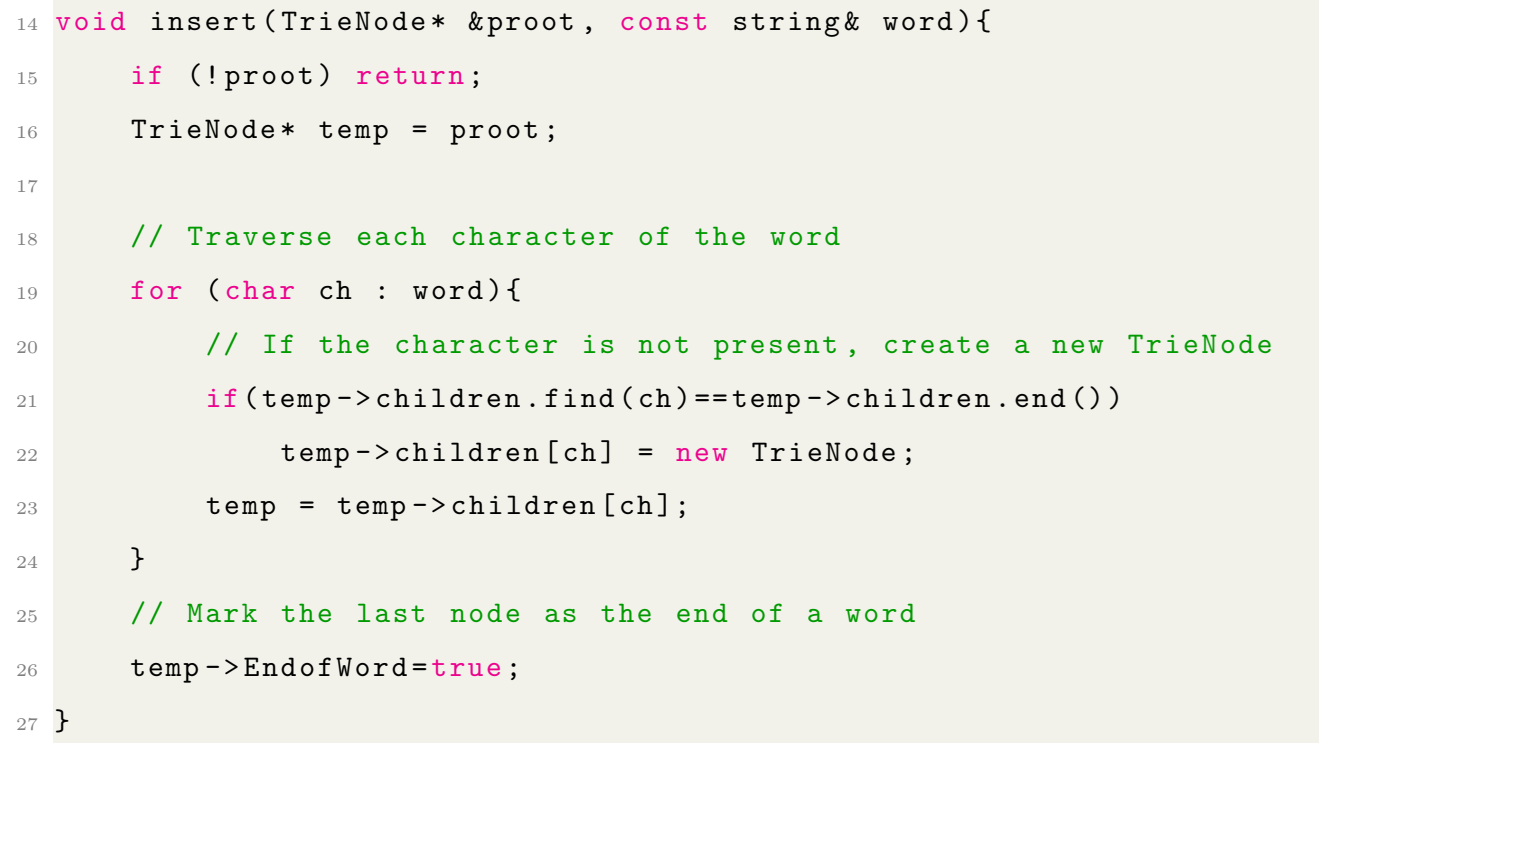
\includegraphics[scale=0.5]{se2.png}
\end{frame}
\begin{frame}{Search "bat"}
    \begin{center}
            \begin{tikzpicture}[scale=0.7]
    % Vẽ hình elips chứa "Root node" tại tọa độ (0,0)
    \node[ellipse, draw, minimum width=2cm, minimum height=1cm] at (1,0) {Root node};
    
    % Vẽ vòng tròn chứa "a" tại (0,-2), không tô màu
     \fill[green] (0,-5) circle (0.5cm);
    \draw (0,-2) circle (0.5cm);
    \node at (0,-2) {\textbf{a}}; % Chữ "a" in đậm ở tâm vòng tròn
    \draw[->] (1,-0.7) -- (0,-1.5); % Mũi tên từ dưới "Root node" tới trên "a"
    
    % Vẽ vòng tròn chứa "p" thứ nhất tại (0,-3.5), không tô màu
    \draw (0,-3.5) circle (0.5cm);
    \node at (0,-3.5) {\textbf{p}}; % Chữ "p" in đậm ở tâm vòng tròn
    \draw[->] (0,-2.5) -- (0,-3); % Mũi tên từ dưới "a" tới trên "p"
    
    % Vẽ vòng tròn chứa "p" thứ hai tại (0,-5), không tô màu
    \draw (0,-5) circle (0.5cm);
    \node at (0,-5) {\textbf{p}}; % Chữ "p" in đậm ở tâm vòng tròn
    \draw[->] (0,-4) -- (0,-4.5); % Mũi tên từ dưới "p" trước tới trên "p"
    
    % Vẽ vòng tròn chứa "l" tại (0,-6.5), không tô màu
    \draw (0,-6.5) circle (0.5cm);
    \node at (0,-6.5) {\textbf{l}}; % Chữ "l" in đậm ở tâm vòng tròn
    \draw[->] (0,-5.5) -- (0,-6); % Mũi tên từ dưới "p" tới trên "l"
    
    % Vẽ vòng tròn chứa "e" tại (0,-8), tô màu xanh dương
    \fill[green] (0,-8) circle (0.5cm); % Tô nền màu xanh dương
    \draw (0,-8) circle (0.5cm); % Vẽ viền vòng tròn
    \node at (0,-8) {\textbf{e}}; % Chữ "e" in đậm ở tâm vòng tròn
    \draw[->] (0,-7) -- (0,-7.5); % Mũi tên từ dưới "l" tới trên "e"

    %b
\draw[red!80, ultra thick] (2.75,-2) circle (0.5cm);
\node at (2.75,-2) {\textbf{b}}; % Chữ "a" in đậm ở tâm vòng tròn
    \draw[->] (1,-0.7) -- (2.75,-1.5); % Mũi tên từ dưới "Root node" tới trên "a"
    %a
    \draw (2.75,-3.5) circle (0.5cm);
    \node at (2.75,-3.5) {\textbf{a}}; % Chữ "a" in đậm ở tâm vòng tròn
    \draw[->] (2.75,-2.5) -- (2.75,-3); % Mũi tên từ dưới "Root node" tới trên
    %s
    \draw (3.5,-5) circle (0.5cm);
    \node at (3.5,-5) {\textbf{s}}; % Chữ "p" in đậm ở tâm vòng tròn
    \draw[->] (2.75,-4) -- (3.5,-4.5); % Mũi tên từ dưới "p" trước tới trên "p"
    %e
    \fill[green] (3.5,-6.5) circle (0.5cm);
     \draw (3.5,-6.5) circle (0.5cm);
    \node at (3.5,-6.5) {\textbf{e}}; % Chữ "l" in đậm ở tâm vòng tròn
    \draw[->] (3.5,-5.5) -- (3.5,-6); % Mũi tên từ dưới "p" tới trên "l"
    %t
    \fill[green] (2,-5) circle (0.5cm);
    \draw (2,-5) circle (0.5cm);
    \node at (2,-5) {\textbf{t}}; % Chữ "p" in đậm ở tâm vòng tròn
    \draw[->] (2.75,-4) -- (2,-4.5); % Mũi tên từ dưới "p" trước tới trên "p"
    %m
    \draw (2,-6.5) circle (0.5cm);
    \node at (2,-6.5) {\textbf{m}}; % Chữ "l" in đậm ở tâm vòng tròn
    \draw[->] (2,-5.5) -- (2,-6); % Mũi tên từ dưới "p" tới trên "l"
    %a
    \draw (02,-8) circle (0.5cm); % Vẽ viền vòng tròn
    \node at (02,-8) {\textbf{a}}; % Chữ "e" in đậm ở tâm vòng tròn
    \draw[->] (02,-7) -- (02,-7.5); % Mũi tên từ dưới "l" tới trên "e"
    %n
    \fill[green] (2,-9.5) circle (0.5cm); % Tô nền màu xanh dương
    \draw (02,-9.5) circle (0.5cm); % Vẽ viền vòng tròn
    \node at (02,-9.5) {\textbf{n}}; % Chữ "e" in đậm ở tâm vòng tròn
    \draw[->] (02,-8.5) -- (02,-9); % Mũi tên từ dưới "l" tới trên "e"
\end{tikzpicture}
    \end{center}
\end{frame}
\begin{frame}{Search "bat"}
    \begin{center}
            \begin{tikzpicture}[scale=0.7]
    % Vẽ hình elips chứa "Root node" tại tọa độ (0,0)
    \node[ellipse, draw, minimum width=2cm, minimum height=1cm] at (1,0) {Root node};
    
    % Vẽ vòng tròn chứa "a" tại (0,-2), không tô màu
     \fill[green] (0,-5) circle (0.5cm);
    \draw (0,-2) circle (0.5cm);
    \node at (0,-2) {\textbf{a}}; % Chữ "a" in đậm ở tâm vòng tròn
    \draw[->] (1,-0.7) -- (0,-1.5); % Mũi tên từ dưới "Root node" tới trên "a"
    
    % Vẽ vòng tròn chứa "p" thứ nhất tại (0,-3.5), không tô màu
    \draw (0,-3.5) circle (0.5cm);
    \node at (0,-3.5) {\textbf{p}}; % Chữ "p" in đậm ở tâm vòng tròn
    \draw[->] (0,-2.5) -- (0,-3); % Mũi tên từ dưới "a" tới trên "p"
    
    % Vẽ vòng tròn chứa "p" thứ hai tại (0,-5), không tô màu
    \draw (0,-5) circle (0.5cm);
    \node at (0,-5) {\textbf{p}}; % Chữ "p" in đậm ở tâm vòng tròn
    \draw[->] (0,-4) -- (0,-4.5); % Mũi tên từ dưới "p" trước tới trên "p"
    
    % Vẽ vòng tròn chứa "l" tại (0,-6.5), không tô màu
    \draw (0,-6.5) circle (0.5cm);
    \node at (0,-6.5) {\textbf{l}}; % Chữ "l" in đậm ở tâm vòng tròn
    \draw[->] (0,-5.5) -- (0,-6); % Mũi tên từ dưới "p" tới trên "l"
    
    % Vẽ vòng tròn chứa "e" tại (0,-8), tô màu xanh dương
    \fill[green] (0,-8) circle (0.5cm); % Tô nền màu xanh dương
    \draw (0,-8) circle (0.5cm); % Vẽ viền vòng tròn
    \node at (0,-8) {\textbf{e}}; % Chữ "e" in đậm ở tâm vòng tròn
    \draw[->] (0,-7) -- (0,-7.5); % Mũi tên từ dưới "l" tới trên "e"

    %b
 \draw (2.75,-2) circle (0.5cm);
\node at (2.75,-2) {\textbf{b}}; % Chữ "a" in đậm ở tâm vòng tròn
    \draw[->] (1,-0.7) -- (2.75,-1.5); % Mũi tên từ dưới "Root node" tới trên "a"
    %a
    \draw[red!80, ultra thick] (2.75,-3.5) circle (0.5cm);
    \node at (2.75,-3.5) {\textbf{a}}; % Chữ "a" in đậm ở tâm vòng tròn
    \draw[->] (2.75,-2.5) -- (2.75,-3); % Mũi tên từ dưới "Root node" tới trên
    %s
    \draw (3.5,-5) circle (0.5cm);
    \node at (3.5,-5) {\textbf{s}}; % Chữ "p" in đậm ở tâm vòng tròn
    \draw[->] (2.75,-4) -- (3.5,-4.5); % Mũi tên từ dưới "p" trước tới trên "p"
    %e
    \fill[green] (3.5,-6.5) circle (0.5cm);
     \draw (3.5,-6.5) circle (0.5cm);
    \node at (3.5,-6.5) {\textbf{e}}; % Chữ "l" in đậm ở tâm vòng tròn
    \draw[->] (3.5,-5.5) -- (3.5,-6); % Mũi tên từ dưới "p" tới trên "l"
    %t
    \fill[green] (2,-5) circle (0.5cm);
    \draw (2,-5) circle (0.5cm);
    \node at (2,-5) {\textbf{t}}; % Chữ "p" in đậm ở tâm vòng tròn
    \draw[->] (2.75,-4) -- (2,-4.5); % Mũi tên từ dưới "p" trước tới trên "p"
    %m
    \draw (2,-6.5) circle (0.5cm);
    \node at (2,-6.5) {\textbf{m}}; % Chữ "l" in đậm ở tâm vòng tròn
    \draw[->] (2,-5.5) -- (2,-6); % Mũi tên từ dưới "p" tới trên "l"
    %a
    \draw (02,-8) circle (0.5cm); % Vẽ viền vòng tròn
    \node at (02,-8) {\textbf{a}}; % Chữ "e" in đậm ở tâm vòng tròn
    \draw[->] (02,-7) -- (02,-7.5); % Mũi tên từ dưới "l" tới trên "e"
    %n
    \fill[green] (2,-9.5) circle (0.5cm); % Tô nền màu xanh dương
    \draw (02,-9.5) circle (0.5cm); % Vẽ viền vòng tròn
    \node at (02,-9.5) {\textbf{n}}; % Chữ "e" in đậm ở tâm vòng tròn
    \draw[->] (02,-8.5) -- (02,-9); % Mũi tên từ dưới "l" tới trên "e"
\end{tikzpicture}
    \end{center}
\end{frame}

\begin{frame}{Search "bat": TRUE}
    \begin{center}
            \begin{tikzpicture}[scale=0.7]
    % Vẽ hình elips chứa "Root node" tại tọa độ (0,0)
    \node[ellipse, draw, minimum width=2cm, minimum height=1cm] at (1,0) {Root node};
    
    % Vẽ vòng tròn chứa "a" tại (0,-2), không tô màu
     \fill[green] (0,-5) circle (0.5cm);
    \draw (0,-2) circle (0.5cm);
    \node at (0,-2) {\textbf{a}}; % Chữ "a" in đậm ở tâm vòng tròn
    \draw[->] (1,-0.7) -- (0,-1.5); % Mũi tên từ dưới "Root node" tới trên "a"
    
    % Vẽ vòng tròn chứa "p" thứ nhất tại (0,-3.5), không tô màu
    \draw (0,-3.5) circle (0.5cm);
    \node at (0,-3.5) {\textbf{p}}; % Chữ "p" in đậm ở tâm vòng tròn
    \draw[->] (0,-2.5) -- (0,-3); % Mũi tên từ dưới "a" tới trên "p"
    
    % Vẽ vòng tròn chứa "p" thứ hai tại (0,-5), không tô màu
    \draw (0,-5) circle (0.5cm);
    \node at (0,-5) {\textbf{p}}; % Chữ "p" in đậm ở tâm vòng tròn
    \draw[->] (0,-4) -- (0,-4.5); % Mũi tên từ dưới "p" trước tới trên "p"
    
    % Vẽ vòng tròn chứa "l" tại (0,-6.5), không tô màu
    \draw (0,-6.5) circle (0.5cm);
    \node at (0,-6.5) {\textbf{l}}; % Chữ "l" in đậm ở tâm vòng tròn
    \draw[->] (0,-5.5) -- (0,-6); % Mũi tên từ dưới "p" tới trên "l"
    
    % Vẽ vòng tròn chứa "e" tại (0,-8), tô màu xanh dương
    \fill[green] (0,-8) circle (0.5cm); % Tô nền màu xanh dương
    \draw (0,-8) circle (0.5cm); % Vẽ viền vòng tròn
    \node at (0,-8) {\textbf{e}}; % Chữ "e" in đậm ở tâm vòng tròn
    \draw[->] (0,-7) -- (0,-7.5); % Mũi tên từ dưới "l" tới trên "e"

    %b
 \draw (2.75,-2) circle (0.5cm);
\node at (2.75,-2) {\textbf{b}}; % Chữ "a" in đậm ở tâm vòng tròn
    \draw[->] (1,-0.7) -- (2.75,-1.5); % Mũi tên từ dưới "Root node" tới trên "a"
    %a
    \draw (2.75,-3.5) circle (0.5cm);
    \node at (2.75,-3.5) {\textbf{a}}; % Chữ "a" in đậm ở tâm vòng tròn
    \draw[->] (2.75,-2.5) -- (2.75,-3); % Mũi tên từ dưới "Root node" tới trên
    %s
    \draw (3.5,-5) circle (0.5cm);
    \node at (3.5,-5) {\textbf{s}}; % Chữ "p" in đậm ở tâm vòng tròn
    \draw[->] (2.75,-4) -- (3.5,-4.5); % Mũi tên từ dưới "p" trước tới trên "p"
    %e
    \fill[green] (3.5,-6.5) circle (0.5cm);
     \draw (3.5,-6.5) circle (0.5cm);
    \node at (3.5,-6.5) {\textbf{e}}; % Chữ "l" in đậm ở tâm vòng tròn
    \draw[->] (3.5,-5.5) -- (3.5,-6); % Mũi tên từ dưới "p" tới trên "l"
    %t
    \fill[green] (2,-5) circle (0.5cm);
    \draw[red!80, ultra thick] (2,-5) circle (0.5cm);
    \node at (2,-5) {\textbf{t}}; % Chữ "p" in đậm ở tâm vòng tròn
    \draw[->] (2.75,-4) -- (2,-4.5); % Mũi tên từ dưới "p" trước tới trên "p"
    %m
    \draw (2,-6.5) circle (0.5cm);
    \node at (2,-6.5) {\textbf{m}}; % Chữ "l" in đậm ở tâm vòng tròn
    \draw[->] (2,-5.5) -- (2,-6); % Mũi tên từ dưới "p" tới trên "l"
    %a
    \draw (02,-8) circle (0.5cm); % Vẽ viền vòng tròn
    \node at (02,-8) {\textbf{a}}; % Chữ "e" in đậm ở tâm vòng tròn
    \draw[->] (02,-7) -- (02,-7.5); % Mũi tên từ dưới "l" tới trên "e"
    %n
    \fill[green] (2,-9.5) circle (0.5cm); % Tô nền màu xanh dương
    \draw (02,-9.5) circle (0.5cm); % Vẽ viền vòng tròn
    \node at (02,-9.5) {\textbf{n}}; % Chữ "e" in đậm ở tâm vòng tròn
    \draw[->] (02,-8.5) -- (02,-9); % Mũi tên từ dưới "l" tới trên "e"
\end{tikzpicture}
    \end{center}
\end{frame}
\begin{frame}{Search "ba"}
    \begin{center}
            \begin{tikzpicture}[scale=0.7]
    % Vẽ hình elips chứa "Root node" tại tọa độ (0,0)
    \node[ellipse, draw, minimum width=2cm, minimum height=1cm] at (1,0) {Root node};
    
    % Vẽ vòng tròn chứa "a" tại (0,-2), không tô màu
     \fill[green] (0,-5) circle (0.5cm);
    \draw (0,-2) circle (0.5cm);
    \node at (0,-2) {\textbf{a}}; % Chữ "a" in đậm ở tâm vòng tròn
    \draw[->] (1,-0.7) -- (0,-1.5); % Mũi tên từ dưới "Root node" tới trên "a"
    
    % Vẽ vòng tròn chứa "p" thứ nhất tại (0,-3.5), không tô màu
    \draw (0,-3.5) circle (0.5cm);
    \node at (0,-3.5) {\textbf{p}}; % Chữ "p" in đậm ở tâm vòng tròn
    \draw[->] (0,-2.5) -- (0,-3); % Mũi tên từ dưới "a" tới trên "p"
    
    % Vẽ vòng tròn chứa "p" thứ hai tại (0,-5), không tô màu
    \draw (0,-5) circle (0.5cm);
    \node at (0,-5) {\textbf{p}}; % Chữ "p" in đậm ở tâm vòng tròn
    \draw[->] (0,-4) -- (0,-4.5); % Mũi tên từ dưới "p" trước tới trên "p"
    
    % Vẽ vòng tròn chứa "l" tại (0,-6.5), không tô màu
    \draw (0,-6.5) circle (0.5cm);
    \node at (0,-6.5) {\textbf{l}}; % Chữ "l" in đậm ở tâm vòng tròn
    \draw[->] (0,-5.5) -- (0,-6); % Mũi tên từ dưới "p" tới trên "l"
    
    % Vẽ vòng tròn chứa "e" tại (0,-8), tô màu xanh dương
    \fill[green] (0,-8) circle (0.5cm); % Tô nền màu xanh dương
    \draw (0,-8) circle (0.5cm); % Vẽ viền vòng tròn
    \node at (0,-8) {\textbf{e}}; % Chữ "e" in đậm ở tâm vòng tròn
    \draw[->] (0,-7) -- (0,-7.5); % Mũi tên từ dưới "l" tới trên "e"

    %b
\draw[red!80, ultra thick] (2.75,-2) circle (0.5cm);
\node at (2.75,-2) {\textbf{b}}; % Chữ "a" in đậm ở tâm vòng tròn
    \draw[->] (1,-0.7) -- (2.75,-1.5); % Mũi tên từ dưới "Root node" tới trên "a"
    %a
    \draw (2.75,-3.5) circle (0.5cm);
    \node at (2.75,-3.5) {\textbf{a}}; % Chữ "a" in đậm ở tâm vòng tròn
    \draw[->] (2.75,-2.5) -- (2.75,-3); % Mũi tên từ dưới "Root node" tới trên
    %s
    \draw (3.5,-5) circle (0.5cm);
    \node at (3.5,-5) {\textbf{s}}; % Chữ "p" in đậm ở tâm vòng tròn
    \draw[->] (2.75,-4) -- (3.5,-4.5); % Mũi tên từ dưới "p" trước tới trên "p"
    %e
    \fill[green] (3.5,-6.5) circle (0.5cm);
     \draw (3.5,-6.5) circle (0.5cm);
    \node at (3.5,-6.5) {\textbf{e}}; % Chữ "l" in đậm ở tâm vòng tròn
    \draw[->] (3.5,-5.5) -- (3.5,-6); % Mũi tên từ dưới "p" tới trên "l"
    %t
    \fill[green] (2,-5) circle (0.5cm);
    \draw (2,-5) circle (0.5cm);
    \node at (2,-5) {\textbf{t}}; % Chữ "p" in đậm ở tâm vòng tròn
    \draw[->] (2.75,-4) -- (2,-4.5); % Mũi tên từ dưới "p" trước tới trên "p"
    %m
    \draw (2,-6.5) circle (0.5cm);
    \node at (2,-6.5) {\textbf{m}}; % Chữ "l" in đậm ở tâm vòng tròn
    \draw[->] (2,-5.5) -- (2,-6); % Mũi tên từ dưới "p" tới trên "l"
    %a
    \draw (02,-8) circle (0.5cm); % Vẽ viền vòng tròn
    \node at (02,-8) {\textbf{a}}; % Chữ "e" in đậm ở tâm vòng tròn
    \draw[->] (02,-7) -- (02,-7.5); % Mũi tên từ dưới "l" tới trên "e"
    %n
    \fill[green] (2,-9.5) circle (0.5cm); % Tô nền màu xanh dương
    \draw (02,-9.5) circle (0.5cm); % Vẽ viền vòng tròn
    \node at (02,-9.5) {\textbf{n}}; % Chữ "e" in đậm ở tâm vòng tròn
    \draw[->] (02,-8.5) -- (02,-9); % Mũi tên từ dưới "l" tới trên "e"
\end{tikzpicture}
    \end{center}
\end{frame}
\begin{frame}{Search "ba": FALSE}
    \begin{center}
            \begin{tikzpicture}[scale=0.7]
    % Vẽ hình elips chứa "Root node" tại tọa độ (0,0)
    \node[ellipse, draw, minimum width=2cm, minimum height=1cm] at (1,0) {Root node};
    
    % Vẽ vòng tròn chứa "a" tại (0,-2), không tô màu
     \fill[green] (0,-5) circle (0.5cm);
    \draw (0,-2) circle (0.5cm);
    \node at (0,-2) {\textbf{a}}; % Chữ "a" in đậm ở tâm vòng tròn
    \draw[->] (1,-0.7) -- (0,-1.5); % Mũi tên từ dưới "Root node" tới trên "a"
    
    % Vẽ vòng tròn chứa "p" thứ nhất tại (0,-3.5), không tô màu
    \draw (0,-3.5) circle (0.5cm);
    \node at (0,-3.5) {\textbf{p}}; % Chữ "p" in đậm ở tâm vòng tròn
    \draw[->] (0,-2.5) -- (0,-3); % Mũi tên từ dưới "a" tới trên "p"
    
    % Vẽ vòng tròn chứa "p" thứ hai tại (0,-5), không tô màu
    \draw (0,-5) circle (0.5cm);
    \node at (0,-5) {\textbf{p}}; % Chữ "p" in đậm ở tâm vòng tròn
    \draw[->] (0,-4) -- (0,-4.5); % Mũi tên từ dưới "p" trước tới trên "p"
    
    % Vẽ vòng tròn chứa "l" tại (0,-6.5), không tô màu
    \draw (0,-6.5) circle (0.5cm);
    \node at (0,-6.5) {\textbf{l}}; % Chữ "l" in đậm ở tâm vòng tròn
    \draw[->] (0,-5.5) -- (0,-6); % Mũi tên từ dưới "p" tới trên "l"
    
    % Vẽ vòng tròn chứa "e" tại (0,-8), tô màu xanh dương
    \fill[green] (0,-8) circle (0.5cm); % Tô nền màu xanh dương
    \draw (0,-8) circle (0.5cm); % Vẽ viền vòng tròn
    \node at (0,-8) {\textbf{e}}; % Chữ "e" in đậm ở tâm vòng tròn
    \draw[->] (0,-7) -- (0,-7.5); % Mũi tên từ dưới "l" tới trên "e"

    %b
 \draw (2.75,-2) circle (0.5cm);
\node at (2.75,-2) {\textbf{b}}; % Chữ "a" in đậm ở tâm vòng tròn
    \draw[->] (1,-0.7) -- (2.75,-1.5); % Mũi tên từ dưới "Root node" tới trên "a"
    %a
    \draw[red!80, ultra thick] (2.75,-3.5) circle (0.5cm);
    \node at (2.75,-3.5) {\textbf{a}}; % Chữ "a" in đậm ở tâm vòng tròn
    \draw[->] (2.75,-2.5) -- (2.75,-3); % Mũi tên từ dưới "Root node" tới trên
    %s
    \draw (3.5,-5) circle (0.5cm);
    \node at (3.5,-5) {\textbf{s}}; % Chữ "p" in đậm ở tâm vòng tròn
    \draw[->] (2.75,-4) -- (3.5,-4.5); % Mũi tên từ dưới "p" trước tới trên "p"
    %e
    \fill[green] (3.5,-6.5) circle (0.5cm);
     \draw (3.5,-6.5) circle (0.5cm);
    \node at (3.5,-6.5) {\textbf{e}}; % Chữ "l" in đậm ở tâm vòng tròn
    \draw[->] (3.5,-5.5) -- (3.5,-6); % Mũi tên từ dưới "p" tới trên "l"
    %t
    \fill[green] (2,-5) circle (0.5cm);
    \draw (2,-5) circle (0.5cm);
    \node at (2,-5) {\textbf{t}}; % Chữ "p" in đậm ở tâm vòng tròn
    \draw[->] (2.75,-4) -- (2,-4.5); % Mũi tên từ dưới "p" trước tới trên "p"
    %m
    \draw (2,-6.5) circle (0.5cm);
    \node at (2,-6.5) {\textbf{m}}; % Chữ "l" in đậm ở tâm vòng tròn
    \draw[->] (2,-5.5) -- (2,-6); % Mũi tên từ dưới "p" tới trên "l"
    %a
    \draw (02,-8) circle (0.5cm); % Vẽ viền vòng tròn
    \node at (02,-8) {\textbf{a}}; % Chữ "e" in đậm ở tâm vòng tròn
    \draw[->] (02,-7) -- (02,-7.5); % Mũi tên từ dưới "l" tới trên "e"
    %n
    \fill[green] (2,-9.5) circle (0.5cm); % Tô nền màu xanh dương
    \draw (02,-9.5) circle (0.5cm); % Vẽ viền vòng tròn
    \node at (02,-9.5) {\textbf{n}}; % Chữ "e" in đậm ở tâm vòng tròn
    \draw[->] (02,-8.5) -- (02,-9); % Mũi tên từ dưới "l" tới trên "e"
\end{tikzpicture}
    \end{center}
\end{frame}

\begin{frame}{Delete: O(L)}
    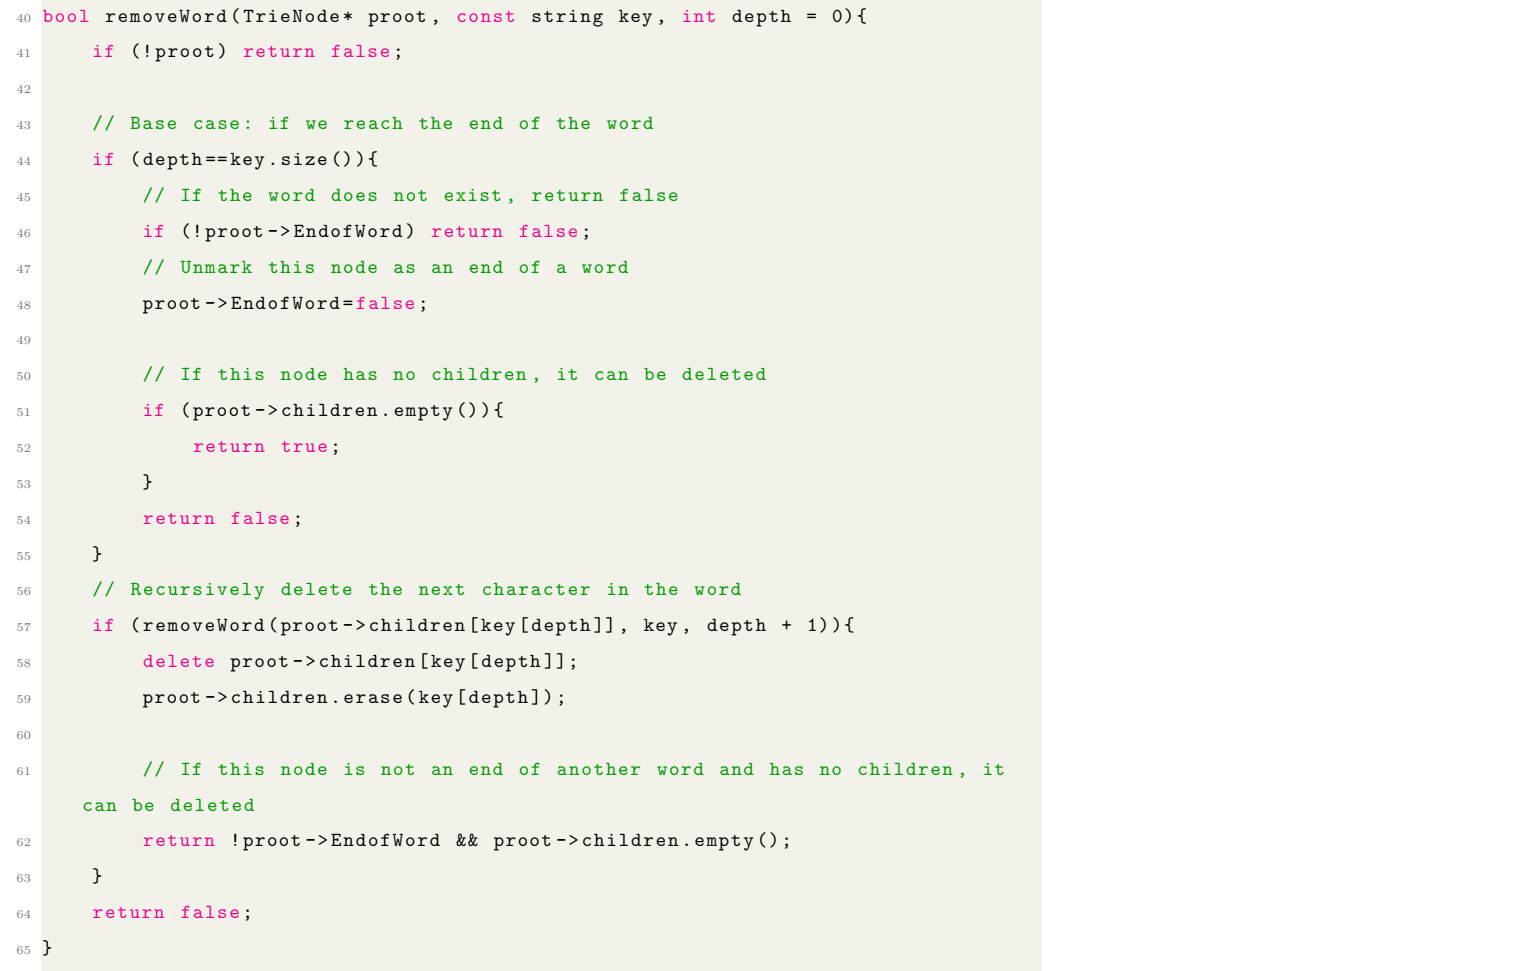
\includegraphics[scale=0.4]{se4.png}
\end{frame}
\begin{frame}{Delete "base"}
    \begin{center}
            \begin{tikzpicture}[scale=0.7]
    % Vẽ hình elips chứa "Root node" tại tọa độ (0,0)
    \node[ellipse, draw, minimum width=2cm, minimum height=1cm] at (1,0) {Root node};
    
    % Vẽ vòng tròn chứa "a" tại (0,-2), không tô màu
     \fill[green] (0,-5) circle (0.5cm);
    \draw (0,-2) circle (0.5cm);
    \node at (0,-2) {\textbf{a}}; % Chữ "a" in đậm ở tâm vòng tròn
    \draw[->] (1,-0.7) -- (0,-1.5); % Mũi tên từ dưới "Root node" tới trên "a"
    
    % Vẽ vòng tròn chứa "p" thứ nhất tại (0,-3.5), không tô màu
    \draw (0,-3.5) circle (0.5cm);
    \node at (0,-3.5) {\textbf{p}}; % Chữ "p" in đậm ở tâm vòng tròn
    \draw[->] (0,-2.5) -- (0,-3); % Mũi tên từ dưới "a" tới trên "p"
    
    % Vẽ vòng tròn chứa "p" thứ hai tại (0,-5), không tô màu
    \draw (0,-5) circle (0.5cm);
    \node at (0,-5) {\textbf{p}}; % Chữ "p" in đậm ở tâm vòng tròn
    \draw[->] (0,-4) -- (0,-4.5); % Mũi tên từ dưới "p" trước tới trên "p"
    
    % Vẽ vòng tròn chứa "l" tại (0,-6.5), không tô màu
    \draw (0,-6.5) circle (0.5cm);
    \node at (0,-6.5) {\textbf{l}}; % Chữ "l" in đậm ở tâm vòng tròn
    \draw[->] (0,-5.5) -- (0,-6); % Mũi tên từ dưới "p" tới trên "l"
    
    % Vẽ vòng tròn chứa "e" tại (0,-8), tô màu xanh dương
    \fill[green] (0,-8) circle (0.5cm); % Tô nền màu xanh dương
    \draw (0,-8) circle (0.5cm); % Vẽ viền vòng tròn
    \node at (0,-8) {\textbf{e}}; % Chữ "e" in đậm ở tâm vòng tròn
    \draw[->] (0,-7) -- (0,-7.5); % Mũi tên từ dưới "l" tới trên "e"

    %b
\draw[red!80, ultra thick] (2.75,-2) circle (0.5cm);
\node at (2.75,-2) {\textbf{b}}; % Chữ "a" in đậm ở tâm vòng tròn
    \draw[->] (1,-0.7) -- (2.75,-1.5); % Mũi tên từ dưới "Root node" tới trên "a"
    %a
    \draw (2.75,-3.5) circle (0.5cm);
    \node at (2.75,-3.5) {\textbf{a}}; % Chữ "a" in đậm ở tâm vòng tròn
    \draw[->] (2.75,-2.5) -- (2.75,-3); % Mũi tên từ dưới "Root node" tới trên
    %s
    \draw (3.5,-5) circle (0.5cm);
    \node at (3.5,-5) {\textbf{s}}; % Chữ "p" in đậm ở tâm vòng tròn
    \draw[->] (2.75,-4) -- (3.5,-4.5); % Mũi tên từ dưới "p" trước tới trên "p"
    %e
    \fill[green] (3.5,-6.5) circle (0.5cm);
     \draw (3.5,-6.5) circle (0.5cm);
    \node at (3.5,-6.5) {\textbf{e}}; % Chữ "l" in đậm ở tâm vòng tròn
    \draw[->] (3.5,-5.5) -- (3.5,-6); % Mũi tên từ dưới "p" tới trên "l"
    %t
    \fill[green] (2,-5) circle (0.5cm);
    \draw (2,-5) circle (0.5cm);
    \node at (2,-5) {\textbf{t}}; % Chữ "p" in đậm ở tâm vòng tròn
    \draw[->] (2.75,-4) -- (2,-4.5); % Mũi tên từ dưới "p" trước tới trên "p"
    %m
    \draw (2,-6.5) circle (0.5cm);
    \node at (2,-6.5) {\textbf{m}}; % Chữ "l" in đậm ở tâm vòng tròn
    \draw[->] (2,-5.5) -- (2,-6); % Mũi tên từ dưới "p" tới trên "l"
    %a
    \draw (02,-8) circle (0.5cm); % Vẽ viền vòng tròn
    \node at (02,-8) {\textbf{a}}; % Chữ "e" in đậm ở tâm vòng tròn
    \draw[->] (02,-7) -- (02,-7.5); % Mũi tên từ dưới "l" tới trên "e"
    %n
    \fill[green] (2,-9.5) circle (0.5cm); % Tô nền màu xanh dương
    \draw (02,-9.5) circle (0.5cm); % Vẽ viền vòng tròn
    \node at (02,-9.5) {\textbf{n}}; % Chữ "e" in đậm ở tâm vòng tròn
    \draw[->] (02,-8.5) -- (02,-9); % Mũi tên từ dưới "l" tới trên "e"
\end{tikzpicture}
    \end{center}
\end{frame}
\begin{frame}{Delete "base"}
    \begin{center}
            \begin{tikzpicture}[scale=0.7]
    % Vẽ hình elips chứa "Root node" tại tọa độ (0,0)
    \node[ellipse, draw, minimum width=2cm, minimum height=1cm] at (1,0) {Root node};
    
    % Vẽ vòng tròn chứa "a" tại (0,-2), không tô màu
     \fill[green] (0,-5) circle (0.5cm);
    \draw (0,-2) circle (0.5cm);
    \node at (0,-2) {\textbf{a}}; % Chữ "a" in đậm ở tâm vòng tròn
    \draw[->] (1,-0.7) -- (0,-1.5); % Mũi tên từ dưới "Root node" tới trên "a"
    
    % Vẽ vòng tròn chứa "p" thứ nhất tại (0,-3.5), không tô màu
    \draw (0,-3.5) circle (0.5cm);
    \node at (0,-3.5) {\textbf{p}}; % Chữ "p" in đậm ở tâm vòng tròn
    \draw[->] (0,-2.5) -- (0,-3); % Mũi tên từ dưới "a" tới trên "p"
    
    % Vẽ vòng tròn chứa "p" thứ hai tại (0,-5), không tô màu
    \draw (0,-5) circle (0.5cm);
    \node at (0,-5) {\textbf{p}}; % Chữ "p" in đậm ở tâm vòng tròn
    \draw[->] (0,-4) -- (0,-4.5); % Mũi tên từ dưới "p" trước tới trên "p"
    
    % Vẽ vòng tròn chứa "l" tại (0,-6.5), không tô màu
    \draw (0,-6.5) circle (0.5cm);
    \node at (0,-6.5) {\textbf{l}}; % Chữ "l" in đậm ở tâm vòng tròn
    \draw[->] (0,-5.5) -- (0,-6); % Mũi tên từ dưới "p" tới trên "l"
    
    % Vẽ vòng tròn chứa "e" tại (0,-8), tô màu xanh dương
    \fill[green] (0,-8) circle (0.5cm); % Tô nền màu xanh dương
    \draw (0,-8) circle (0.5cm); % Vẽ viền vòng tròn
    \node at (0,-8) {\textbf{e}}; % Chữ "e" in đậm ở tâm vòng tròn
    \draw[->] (0,-7) -- (0,-7.5); % Mũi tên từ dưới "l" tới trên "e"

    %b
 \draw (2.75,-2) circle (0.5cm);
\node at (2.75,-2) {\textbf{b}}; % Chữ "a" in đậm ở tâm vòng tròn
    \draw[->] (1,-0.7) -- (2.75,-1.5); % Mũi tên từ dưới "Root node" tới trên "a"
    %a
    \draw[red!80, ultra thick] (2.75,-3.5) circle (0.5cm);
    \node at (2.75,-3.5) {\textbf{a}}; % Chữ "a" in đậm ở tâm vòng tròn
    \draw[->] (2.75,-2.5) -- (2.75,-3); % Mũi tên từ dưới "Root node" tới trên
    %s
    \draw (3.5,-5) circle (0.5cm);
    \node at (3.5,-5) {\textbf{s}}; % Chữ "p" in đậm ở tâm vòng tròn
    \draw[->] (2.75,-4) -- (3.5,-4.5); % Mũi tên từ dưới "p" trước tới trên "p"
    %e
    \fill[green] (3.5,-6.5) circle (0.5cm);
     \draw (3.5,-6.5) circle (0.5cm);
    \node at (3.5,-6.5) {\textbf{e}}; % Chữ "l" in đậm ở tâm vòng tròn
    \draw[->] (3.5,-5.5) -- (3.5,-6); % Mũi tên từ dưới "p" tới trên "l"
    %t
    \fill[green] (2,-5) circle (0.5cm);
    \draw (2,-5) circle (0.5cm);
    \node at (2,-5) {\textbf{t}}; % Chữ "p" in đậm ở tâm vòng tròn
    \draw[->] (2.75,-4) -- (2,-4.5); % Mũi tên từ dưới "p" trước tới trên "p"
    %m
    \draw (2,-6.5) circle (0.5cm);
    \node at (2,-6.5) {\textbf{m}}; % Chữ "l" in đậm ở tâm vòng tròn
    \draw[->] (2,-5.5) -- (2,-6); % Mũi tên từ dưới "p" tới trên "l"
    %a
    \draw (02,-8) circle (0.5cm); % Vẽ viền vòng tròn
    \node at (02,-8) {\textbf{a}}; % Chữ "e" in đậm ở tâm vòng tròn
    \draw[->] (02,-7) -- (02,-7.5); % Mũi tên từ dưới "l" tới trên "e"
    %n
    \fill[green] (2,-9.5) circle (0.5cm); % Tô nền màu xanh dương
    \draw (02,-9.5) circle (0.5cm); % Vẽ viền vòng tròn
    \node at (02,-9.5) {\textbf{n}}; % Chữ "e" in đậm ở tâm vòng tròn
    \draw[->] (02,-8.5) -- (02,-9); % Mũi tên từ dưới "l" tới trên "e"
\end{tikzpicture}
    \end{center}
\end{frame}
\begin{frame}{Delete "base"}
    \begin{center}
            \begin{tikzpicture}[scale=0.7]
    % Vẽ hình elips chứa "Root node" tại tọa độ (0,0)
    \node[ellipse, draw, minimum width=2cm, minimum height=1cm] at (1,0) {Root node};
    
    % Vẽ vòng tròn chứa "a" tại (0,-2), không tô màu
     \fill[green] (0,-5) circle (0.5cm);
    \draw (0,-2) circle (0.5cm);
    \node at (0,-2) {\textbf{a}}; % Chữ "a" in đậm ở tâm vòng tròn
    \draw[->] (1,-0.7) -- (0,-1.5); % Mũi tên từ dưới "Root node" tới trên "a"
    
    % Vẽ vòng tròn chứa "p" thứ nhất tại (0,-3.5), không tô màu
    \draw (0,-3.5) circle (0.5cm);
    \node at (0,-3.5) {\textbf{p}}; % Chữ "p" in đậm ở tâm vòng tròn
    \draw[->] (0,-2.5) -- (0,-3); % Mũi tên từ dưới "a" tới trên "p"
    
    % Vẽ vòng tròn chứa "p" thứ hai tại (0,-5), không tô màu
    \draw (0,-5) circle (0.5cm);
    \node at (0,-5) {\textbf{p}}; % Chữ "p" in đậm ở tâm vòng tròn
    \draw[->] (0,-4) -- (0,-4.5); % Mũi tên từ dưới "p" trước tới trên "p"
    
    % Vẽ vòng tròn chứa "l" tại (0,-6.5), không tô màu
    \draw (0,-6.5) circle (0.5cm);
    \node at (0,-6.5) {\textbf{l}}; % Chữ "l" in đậm ở tâm vòng tròn
    \draw[->] (0,-5.5) -- (0,-6); % Mũi tên từ dưới "p" tới trên "l"
    
    % Vẽ vòng tròn chứa "e" tại (0,-8), tô màu xanh dương
    \fill[green] (0,-8) circle (0.5cm); % Tô nền màu xanh dương
    \draw (0,-8) circle (0.5cm); % Vẽ viền vòng tròn
    \node at (0,-8) {\textbf{e}}; % Chữ "e" in đậm ở tâm vòng tròn
    \draw[->] (0,-7) -- (0,-7.5); % Mũi tên từ dưới "l" tới trên "e"

    %b
 \draw (2.75,-2) circle (0.5cm);
\node at (2.75,-2) {\textbf{b}}; % Chữ "a" in đậm ở tâm vòng tròn
    \draw[->] (1,-0.7) -- (2.75,-1.5); % Mũi tên từ dưới "Root node" tới trên "a"
    %a
    \draw (2.75,-3.5) circle (0.5cm);
    \node at (2.75,-3.5) {\textbf{a}}; % Chữ "a" in đậm ở tâm vòng tròn
    \draw[->] (2.75,-2.5) -- (2.75,-3); % Mũi tên từ dưới "Root node" tới trên
    %s
    \draw[red!80, ultra thick] (3.5,-5) circle (0.5cm);
    \node at (3.5,-5) {\textbf{s}}; % Chữ "p" in đậm ở tâm vòng tròn
    \draw[->] (2.75,-4) -- (3.5,-4.5); % Mũi tên từ dưới "p" trước tới trên "p"
    %e
    \fill[green] (3.5,-6.5) circle (0.5cm);
     \draw (3.5,-6.5) circle (0.5cm);
    \node at (3.5,-6.5) {\textbf{e}}; % Chữ "l" in đậm ở tâm vòng tròn
    \draw[->] (3.5,-5.5) -- (3.5,-6); % Mũi tên từ dưới "p" tới trên "l"
    %t
    \fill[green] (2,-5) circle (0.5cm);
    \draw (2,-5) circle (0.5cm);
    \node at (2,-5) {\textbf{t}}; % Chữ "p" in đậm ở tâm vòng tròn
    \draw[->] (2.75,-4) -- (2,-4.5); % Mũi tên từ dưới "p" trước tới trên "p"
    %m
    \draw (2,-6.5) circle (0.5cm);
    \node at (2,-6.5) {\textbf{m}}; % Chữ "l" in đậm ở tâm vòng tròn
    \draw[->] (2,-5.5) -- (2,-6); % Mũi tên từ dưới "p" tới trên "l"
    %a
    \draw (02,-8) circle (0.5cm); % Vẽ viền vòng tròn
    \node at (02,-8) {\textbf{a}}; % Chữ "e" in đậm ở tâm vòng tròn
    \draw[->] (02,-7) -- (02,-7.5); % Mũi tên từ dưới "l" tới trên "e"
    %n
    \fill[green] (2,-9.5) circle (0.5cm); % Tô nền màu xanh dương
    \draw (02,-9.5) circle (0.5cm); % Vẽ viền vòng tròn
    \node at (02,-9.5) {\textbf{n}}; % Chữ "e" in đậm ở tâm vòng tròn
    \draw[->] (02,-8.5) -- (02,-9); % Mũi tên từ dưới "l" tới trên "e"
\end{tikzpicture}
    \end{center}
\end{frame}

\begin{frame}{Delete "base"}
    \begin{center}
            \begin{tikzpicture}[scale=0.7]
    % Vẽ hình elips chứa "Root node" tại tọa độ (0,0)
    \node[ellipse, draw, minimum width=2cm, minimum height=1cm] at (1,0) {Root node};
    
    % Vẽ vòng tròn chứa "a" tại (0,-2), không tô màu
     \fill[green] (0,-5) circle (0.5cm);
    \draw (0,-2) circle (0.5cm);
    \node at (0,-2) {\textbf{a}}; % Chữ "a" in đậm ở tâm vòng tròn
    \draw[->] (1,-0.7) -- (0,-1.5); % Mũi tên từ dưới "Root node" tới trên "a"
    
    % Vẽ vòng tròn chứa "p" thứ nhất tại (0,-3.5), không tô màu
    \draw (0,-3.5) circle (0.5cm);
    \node at (0,-3.5) {\textbf{p}}; % Chữ "p" in đậm ở tâm vòng tròn
    \draw[->] (0,-2.5) -- (0,-3); % Mũi tên từ dưới "a" tới trên "p"
    
    % Vẽ vòng tròn chứa "p" thứ hai tại (0,-5), không tô màu
    \draw (0,-5) circle (0.5cm);
    \node at (0,-5) {\textbf{p}}; % Chữ "p" in đậm ở tâm vòng tròn
    \draw[->] (0,-4) -- (0,-4.5); % Mũi tên từ dưới "p" trước tới trên "p"
    
    % Vẽ vòng tròn chứa "l" tại (0,-6.5), không tô màu
    \draw (0,-6.5) circle (0.5cm);
    \node at (0,-6.5) {\textbf{l}}; % Chữ "l" in đậm ở tâm vòng tròn
    \draw[->] (0,-5.5) -- (0,-6); % Mũi tên từ dưới "p" tới trên "l"
    
    % Vẽ vòng tròn chứa "e" tại (0,-8), tô màu xanh dương
    \fill[green] (0,-8) circle (0.5cm); % Tô nền màu xanh dương
    \draw (0,-8) circle (0.5cm); % Vẽ viền vòng tròn
    \node at (0,-8) {\textbf{e}}; % Chữ "e" in đậm ở tâm vòng tròn
    \draw[->] (0,-7) -- (0,-7.5); % Mũi tên từ dưới "l" tới trên "e"

    %b
 \draw (2.75,-2) circle (0.5cm);
\node at (2.75,-2) {\textbf{b}}; % Chữ "a" in đậm ở tâm vòng tròn
    \draw[->] (1,-0.7) -- (2.75,-1.5); % Mũi tên từ dưới "Root node" tới trên "a"
    %a
    \draw (2.75,-3.5) circle (0.5cm);
    \node at (2.75,-3.5) {\textbf{a}}; % Chữ "a" in đậm ở tâm vòng tròn
    \draw[->] (2.75,-2.5) -- (2.75,-3); % Mũi tên từ dưới "Root node" tới trên
    %s
    \draw (3.5,-5) circle (0.5cm);
    \node at (3.5,-5) {\textbf{s}}; % Chữ "p" in đậm ở tâm vòng tròn
    \draw[->] (2.75,-4) -- (3.5,-4.5); % Mũi tên từ dưới "p" trước tới trên "p"
    %e
    \fill[green] (3.5,-6.5) circle (0.5cm);
     \draw[red!80, ultra thick] (3.5,-6.5) circle (0.5cm);
    \node at (3.5,-6.5) {\textbf{e}}; % Chữ "l" in đậm ở tâm vòng tròn
    \draw[->] (3.5,-5.5) -- (3.5,-6); % Mũi tên từ dưới "p" tới trên "l"
    %t
    \fill[green] (2,-5) circle (0.5cm);
    \draw (2,-5) circle (0.5cm);
    \node at (2,-5) {\textbf{t}}; % Chữ "p" in đậm ở tâm vòng tròn
    \draw[->] (2.75,-4) -- (2,-4.5); % Mũi tên từ dưới "p" trước tới trên "p"
    %m
    \draw (2,-6.5) circle (0.5cm);
    \node at (2,-6.5) {\textbf{m}}; % Chữ "l" in đậm ở tâm vòng tròn
    \draw[->] (2,-5.5) -- (2,-6); % Mũi tên từ dưới "p" tới trên "l"
    %a
    \draw (02,-8) circle (0.5cm); % Vẽ viền vòng tròn
    \node at (02,-8) {\textbf{a}}; % Chữ "e" in đậm ở tâm vòng tròn
    \draw[->] (02,-7) -- (02,-7.5); % Mũi tên từ dưới "l" tới trên "e"
    %n
    \fill[green] (2,-9.5) circle (0.5cm); % Tô nền màu xanh dương
    \draw (02,-9.5) circle (0.5cm); % Vẽ viền vòng tròn
    \node at (02,-9.5) {\textbf{n}}; % Chữ "e" in đậm ở tâm vòng tròn
    \draw[->] (02,-8.5) -- (02,-9); % Mũi tên từ dưới "l" tới trên "e"
\end{tikzpicture}
    \end{center}
\end{frame}

\begin{frame}{Delete "base"}
    \begin{center}
            \begin{tikzpicture}[scale=0.7]
    % Vẽ hình elips chứa "Root node" tại tọa độ (0,0)
    \node[ellipse, draw, minimum width=2cm, minimum height=1cm] at (1,0) {Root node};
    
    % Vẽ vòng tròn chứa "a" tại (0,-2), không tô màu
     \fill[green] (0,-5) circle (0.5cm);
    \draw (0,-2) circle (0.5cm);
    \node at (0,-2) {\textbf{a}}; % Chữ "a" in đậm ở tâm vòng tròn
    \draw[->] (1,-0.7) -- (0,-1.5); % Mũi tên từ dưới "Root node" tới trên "a"
    
    % Vẽ vòng tròn chứa "p" thứ nhất tại (0,-3.5), không tô màu
    \draw (0,-3.5) circle (0.5cm);
    \node at (0,-3.5) {\textbf{p}}; % Chữ "p" in đậm ở tâm vòng tròn
    \draw[->] (0,-2.5) -- (0,-3); % Mũi tên từ dưới "a" tới trên "p"
    
    % Vẽ vòng tròn chứa "p" thứ hai tại (0,-5), không tô màu
    \draw (0,-5) circle (0.5cm);
    \node at (0,-5) {\textbf{p}}; % Chữ "p" in đậm ở tâm vòng tròn
    \draw[->] (0,-4) -- (0,-4.5); % Mũi tên từ dưới "p" trước tới trên "p"
    
    % Vẽ vòng tròn chứa "l" tại (0,-6.5), không tô màu
    \draw (0,-6.5) circle (0.5cm);
    \node at (0,-6.5) {\textbf{l}}; % Chữ "l" in đậm ở tâm vòng tròn
    \draw[->] (0,-5.5) -- (0,-6); % Mũi tên từ dưới "p" tới trên "l"
    
    % Vẽ vòng tròn chứa "e" tại (0,-8), tô màu xanh dương
    \fill[green] (0,-8) circle (0.5cm); % Tô nền màu xanh dương
    \draw (0,-8) circle (0.5cm); % Vẽ viền vòng tròn
    \node at (0,-8) {\textbf{e}}; % Chữ "e" in đậm ở tâm vòng tròn
    \draw[->] (0,-7) -- (0,-7.5); % Mũi tên từ dưới "l" tới trên "e"

    %b
 \draw (2.75,-2) circle (0.5cm);
\node at (2.75,-2) {\textbf{b}}; % Chữ "a" in đậm ở tâm vòng tròn
    \draw[->] (1,-0.7) -- (2.75,-1.5); % Mũi tên từ dưới "Root node" tới trên "a"
    %a
    \draw (2.75,-3.5) circle (0.5cm);
    \node at (2.75,-3.5) {\textbf{a}}; % Chữ "a" in đậm ở tâm vòng tròn
    \draw[->] (2.75,-2.5) -- (2.75,-3); % Mũi tên từ dưới "Root node" tới trên
    %s
    \draw[red!80, ultra thick] (3.5,-5) circle (0.5cm);
    \node at (3.5,-5) {\textbf{s}}; % Chữ "p" in đậm ở tâm vòng tròn
    \draw[->] (2.75,-4) -- (3.5,-4.5); % Mũi tên từ dưới "p" trước tới trên "p"
    %t
    \fill[green] (2,-5) circle (0.5cm);
    \draw (2,-5) circle (0.5cm);
    \node at (2,-5) {\textbf{t}}; % Chữ "p" in đậm ở tâm vòng tròn
    \draw[->] (2.75,-4) -- (2,-4.5); % Mũi tên từ dưới "p" trước tới trên "p"
    %m
    \draw (2,-6.5) circle (0.5cm);
    \node at (2,-6.5) {\textbf{m}}; % Chữ "l" in đậm ở tâm vòng tròn
    \draw[->] (2,-5.5) -- (2,-6); % Mũi tên từ dưới "p" tới trên "l"
    %a
    \draw (02,-8) circle (0.5cm); % Vẽ viền vòng tròn
    \node at (02,-8) {\textbf{a}}; % Chữ "e" in đậm ở tâm vòng tròn
    \draw[->] (02,-7) -- (02,-7.5); % Mũi tên từ dưới "l" tới trên "e"
    %n
    \fill[green] (2,-9.5) circle (0.5cm); % Tô nền màu xanh dương
    \draw (02,-9.5) circle (0.5cm); % Vẽ viền vòng tròn
    \node at (02,-9.5) {\textbf{n}}; % Chữ "e" in đậm ở tâm vòng tròn
    \draw[->] (02,-8.5) -- (02,-9); % Mũi tên từ dưới "l" tới trên "e"
\end{tikzpicture}
    \end{center}
\end{frame}

\begin{frame}{Delete "base"}
    \begin{center}
            \begin{tikzpicture}[scale=0.7]
    % Vẽ hình elips chứa "Root node" tại tọa độ (0,0)
    \node[ellipse, draw, minimum width=2cm, minimum height=1cm] at (1,0) {Root node};
    
    % Vẽ vòng tròn chứa "a" tại (0,-2), không tô màu
     \fill[green] (0,-5) circle (0.5cm);
    \draw (0,-2) circle (0.5cm);
    \node at (0,-2) {\textbf{a}}; % Chữ "a" in đậm ở tâm vòng tròn
    \draw[->] (1,-0.7) -- (0,-1.5); % Mũi tên từ dưới "Root node" tới trên "a"
    
    % Vẽ vòng tròn chứa "p" thứ nhất tại (0,-3.5), không tô màu
    \draw (0,-3.5) circle (0.5cm);
    \node at (0,-3.5) {\textbf{p}}; % Chữ "p" in đậm ở tâm vòng tròn
    \draw[->] (0,-2.5) -- (0,-3); % Mũi tên từ dưới "a" tới trên "p"
    
    % Vẽ vòng tròn chứa "p" thứ hai tại (0,-5), không tô màu
    \draw (0,-5) circle (0.5cm);
    \node at (0,-5) {\textbf{p}}; % Chữ "p" in đậm ở tâm vòng tròn
    \draw[->] (0,-4) -- (0,-4.5); % Mũi tên từ dưới "p" trước tới trên "p"
    
    % Vẽ vòng tròn chứa "l" tại (0,-6.5), không tô màu
    \draw (0,-6.5) circle (0.5cm);
    \node at (0,-6.5) {\textbf{l}}; % Chữ "l" in đậm ở tâm vòng tròn
    \draw[->] (0,-5.5) -- (0,-6); % Mũi tên từ dưới "p" tới trên "l"
    
    % Vẽ vòng tròn chứa "e" tại (0,-8), tô màu xanh dương
    \fill[green] (0,-8) circle (0.5cm); % Tô nền màu xanh dương
    \draw (0,-8) circle (0.5cm); % Vẽ viền vòng tròn
    \node at (0,-8) {\textbf{e}}; % Chữ "e" in đậm ở tâm vòng tròn
    \draw[->] (0,-7) -- (0,-7.5); % Mũi tên từ dưới "l" tới trên "e"

    %b
 \draw (2.75,-2) circle (0.5cm);
\node at (2.75,-2) {\textbf{b}}; % Chữ "a" in đậm ở tâm vòng tròn
    \draw[->] (1,-0.7) -- (2.75,-1.5); % Mũi tên từ dưới "Root node" tới trên "a"
    %a
    \draw[red!80, ultra thick]  (2.75,-3.5) circle (0.5cm);
    \node at (2.75,-3.5) {\textbf{a}}; % Chữ "a" in đậm ở tâm vòng tròn
    \draw[->] (2.75,-2.5) -- (2.75,-3); % Mũi tên từ dưới "Root node" tới trên
    %t
    \fill[green] (2,-5) circle (0.5cm);
    \draw (2,-5) circle (0.5cm);
    \node at (2,-5) {\textbf{t}}; % Chữ "p" in đậm ở tâm vòng tròn
    \draw[->] (2.75,-4) -- (2,-4.5); % Mũi tên từ dưới "p" trước tới trên "p"
    %m
    \draw (2,-6.5) circle (0.5cm);
    \node at (2,-6.5) {\textbf{m}}; % Chữ "l" in đậm ở tâm vòng tròn
    \draw[->] (2,-5.5) -- (2,-6); % Mũi tên từ dưới "p" tới trên "l"
    %a
    \draw (02,-8) circle (0.5cm); % Vẽ viền vòng tròn
    \node at (02,-8) {\textbf{a}}; % Chữ "e" in đậm ở tâm vòng tròn
    \draw[->] (02,-7) -- (02,-7.5); % Mũi tên từ dưới "l" tới trên "e"
    %n
    \fill[green] (2,-9.5) circle (0.5cm); % Tô nền màu xanh dương
    \draw (02,-9.5) circle (0.5cm); % Vẽ viền vòng tròn
    \node at (02,-9.5) {\textbf{n}}; % Chữ "e" in đậm ở tâm vòng tròn
    \draw[->] (02,-8.5) -- (02,-9); % Mũi tên từ dưới "l" tới trên "e"
\end{tikzpicture}
    \end{center}
\end{frame}
\begin{frame}{Insert "batman"}
\begin{center}
    \begin{tikzpicture}[scale=0.7]
    % Vẽ hình elips chứa "Root node" tại tọa độ (0,0)
    \node[ellipse, draw, minimum width=2cm, minimum height=1cm] at (1,0) {Root node};
    
    % Vẽ vòng tròn chứa "a" tại (0,-2), không tô màu
     \fill[green] (0,-5) circle (0.5cm);
    \draw (0,-2) circle (0.5cm);
    \node at (0,-2) {\textbf{a}}; % Chữ "a" in đậm ở tâm vòng tròn
    \draw[->] (1,-0.7) -- (0,-1.5); % Mũi tên từ dưới "Root node" tới trên "a"
    
    % Vẽ vòng tròn chứa "p" thứ nhất tại (0,-3.5), không tô màu
    \draw (0,-3.5) circle (0.5cm);
    \node at (0,-3.5) {\textbf{p}}; % Chữ "p" in đậm ở tâm vòng tròn
    \draw[->] (0,-2.5) -- (0,-3); % Mũi tên từ dưới "a" tới trên "p"
    
    % Vẽ vòng tròn chứa "p" thứ hai tại (0,-5), không tô màu
    \draw (0,-5) circle (0.5cm);
    \node at (0,-5) {\textbf{p}}; % Chữ "p" in đậm ở tâm vòng tròn
    \draw[->] (0,-4) -- (0,-4.5); % Mũi tên từ dưới "p" trước tới trên "p"
    
    % Vẽ vòng tròn chứa "l" tại (0,-6.5), không tô màu
    \draw (0,-6.5) circle (0.5cm);
    \node at (0,-6.5) {\textbf{l}}; % Chữ "l" in đậm ở tâm vòng tròn
    \draw[->] (0,-5.5) -- (0,-6); % Mũi tên từ dưới "p" tới trên "l"
    
    % Vẽ vòng tròn chứa "e" tại (0,-8), tô màu xanh dương
    \fill[green] (0,-8) circle (0.5cm); % Tô nền màu xanh dương
    \draw (0,-8) circle (0.5cm); % Vẽ viền vòng tròn
    \node at (0,-8) {\textbf{e}}; % Chữ "e" in đậm ở tâm vòng tròn
    \draw[->] (0,-7) -- (0,-7.5); % Mũi tên từ dưới "l" tới trên "e"

    %b
    \draw (2,-2) circle (0.5cm);
    \node at (2,-2) {\textbf{b}}; % Chữ "a" in đậm ở tâm vòng tròn
    \draw[->] (1,-0.7) -- (2,-1.5); % Mũi tên từ dưới "Root node" tới trên "a"
    %a
    \draw (2,-3.5) circle (0.5cm);
    \node at (2,-3.5) {\textbf{a}}; % Chữ "a" in đậm ở tâm vòng tròn
    \draw[->] (2,-2.5) -- (2,-3); % Mũi tên từ dưới "Root node" tới trên "a"
    %t
    \fill[green] (2,-5) circle (0.5cm);
    \draw (2,-5) circle (0.5cm);
    \node at (2,-5) {\textbf{t}}; % Chữ "p" in đậm ở tâm vòng tròn
    \draw[->] (2,-4) -- (2,-4.5); % Mũi tên từ dưới "p" trước tới trên "p"
    %m
    \draw (2,-6.5) circle (0.5cm);
    \node at (2,-6.5) {\textbf{m}}; % Chữ "l" in đậm ở tâm vòng tròn
    \draw[->] (2,-5.5) -- (2,-6); % Mũi tên từ dưới "p" tới trên "l"
    %a
    \draw (02,-8) circle (0.5cm); % Vẽ viền vòng tròn
    \node at (02,-8) {\textbf{a}}; % Chữ "e" in đậm ở tâm vòng tròn
    \draw[->] (02,-7) -- (02,-7.5); % Mũi tên từ dưới "l" tới trên "e"
    %n
    \fill[green] (2,-9.5) circle (0.5cm); % Tô nền màu xanh dương
    \draw (02,-9.5) circle (0.5cm); % Vẽ viền vòng tròn
    \node at (02,-9.5) {\textbf{n}}; % Chữ "e" in đậm ở tâm vòng tròn
    \draw[->] (02,-8.5) -- (02,-9); % Mũi tên từ dưới "l" tới trên "e"
\end{tikzpicture}
\end{center}
\end{frame}

\begin{frame}{Space Complexity}
    $O(N * M)$, where $N$ is the number of words and $M$ is the average word length. Each character across all words requires a node (or a slot in a dictionary/array), causing the space to scale with the total number of characters stored.
\end{frame}
